% Options for packages loaded elsewhere
\PassOptionsToPackage{unicode}{hyperref}
\PassOptionsToPackage{hyphens}{url}
%
\documentclass[
  8pt,
  ignorenonframetext,
]{beamer}
\usepackage{pgfpages}
\setbeamertemplate{caption}[numbered]
\setbeamertemplate{caption label separator}{: }
\setbeamercolor{caption name}{fg=normal text.fg}
\beamertemplatenavigationsymbolsempty
% Prevent slide breaks in the middle of a paragraph
\widowpenalties 1 10000
\raggedbottom
\setbeamertemplate{part page}{
  \centering
  \begin{beamercolorbox}[sep=16pt,center]{part title}
    \usebeamerfont{part title}\insertpart\par
  \end{beamercolorbox}
}
\setbeamertemplate{section page}{
  \centering
  \begin{beamercolorbox}[sep=12pt,center]{part title}
    \usebeamerfont{section title}\insertsection\par
  \end{beamercolorbox}
}
\setbeamertemplate{subsection page}{
  \centering
  \begin{beamercolorbox}[sep=8pt,center]{part title}
    \usebeamerfont{subsection title}\insertsubsection\par
  \end{beamercolorbox}
}
\AtBeginPart{
  \frame{\partpage}
}
\AtBeginSection{
  \ifbibliography
  \else
    \frame{\sectionpage}
  \fi
}
\AtBeginSubsection{
  \frame{\subsectionpage}
}
\usepackage{amsmath,amssymb}
\usepackage{lmodern}
\usepackage{iftex}
\ifPDFTeX
  \usepackage[T1]{fontenc}
  \usepackage[utf8]{inputenc}
  \usepackage{textcomp} % provide euro and other symbols
\else % if luatex or xetex
  \usepackage{unicode-math}
  \defaultfontfeatures{Scale=MatchLowercase}
  \defaultfontfeatures[\rmfamily]{Ligatures=TeX,Scale=1}
\fi
% Use upquote if available, for straight quotes in verbatim environments
\IfFileExists{upquote.sty}{\usepackage{upquote}}{}
\IfFileExists{microtype.sty}{% use microtype if available
  \usepackage[]{microtype}
  \UseMicrotypeSet[protrusion]{basicmath} % disable protrusion for tt fonts
}{}
\makeatletter
\@ifundefined{KOMAClassName}{% if non-KOMA class
  \IfFileExists{parskip.sty}{%
    \usepackage{parskip}
  }{% else
    \setlength{\parindent}{0pt}
    \setlength{\parskip}{6pt plus 2pt minus 1pt}}
}{% if KOMA class
  \KOMAoptions{parskip=half}}
\makeatother
\usepackage{xcolor}
\newif\ifbibliography
\usepackage{color}
\usepackage{fancyvrb}
\newcommand{\VerbBar}{|}
\newcommand{\VERB}{\Verb[commandchars=\\\{\}]}
\DefineVerbatimEnvironment{Highlighting}{Verbatim}{commandchars=\\\{\}}
% Add ',fontsize=\small' for more characters per line
\usepackage{framed}
\definecolor{shadecolor}{RGB}{248,248,248}
\newenvironment{Shaded}{\begin{snugshade}}{\end{snugshade}}
\newcommand{\AlertTok}[1]{\textcolor[rgb]{0.94,0.16,0.16}{#1}}
\newcommand{\AnnotationTok}[1]{\textcolor[rgb]{0.56,0.35,0.01}{\textbf{\textit{#1}}}}
\newcommand{\AttributeTok}[1]{\textcolor[rgb]{0.77,0.63,0.00}{#1}}
\newcommand{\BaseNTok}[1]{\textcolor[rgb]{0.00,0.00,0.81}{#1}}
\newcommand{\BuiltInTok}[1]{#1}
\newcommand{\CharTok}[1]{\textcolor[rgb]{0.31,0.60,0.02}{#1}}
\newcommand{\CommentTok}[1]{\textcolor[rgb]{0.56,0.35,0.01}{\textit{#1}}}
\newcommand{\CommentVarTok}[1]{\textcolor[rgb]{0.56,0.35,0.01}{\textbf{\textit{#1}}}}
\newcommand{\ConstantTok}[1]{\textcolor[rgb]{0.00,0.00,0.00}{#1}}
\newcommand{\ControlFlowTok}[1]{\textcolor[rgb]{0.13,0.29,0.53}{\textbf{#1}}}
\newcommand{\DataTypeTok}[1]{\textcolor[rgb]{0.13,0.29,0.53}{#1}}
\newcommand{\DecValTok}[1]{\textcolor[rgb]{0.00,0.00,0.81}{#1}}
\newcommand{\DocumentationTok}[1]{\textcolor[rgb]{0.56,0.35,0.01}{\textbf{\textit{#1}}}}
\newcommand{\ErrorTok}[1]{\textcolor[rgb]{0.64,0.00,0.00}{\textbf{#1}}}
\newcommand{\ExtensionTok}[1]{#1}
\newcommand{\FloatTok}[1]{\textcolor[rgb]{0.00,0.00,0.81}{#1}}
\newcommand{\FunctionTok}[1]{\textcolor[rgb]{0.00,0.00,0.00}{#1}}
\newcommand{\ImportTok}[1]{#1}
\newcommand{\InformationTok}[1]{\textcolor[rgb]{0.56,0.35,0.01}{\textbf{\textit{#1}}}}
\newcommand{\KeywordTok}[1]{\textcolor[rgb]{0.13,0.29,0.53}{\textbf{#1}}}
\newcommand{\NormalTok}[1]{#1}
\newcommand{\OperatorTok}[1]{\textcolor[rgb]{0.81,0.36,0.00}{\textbf{#1}}}
\newcommand{\OtherTok}[1]{\textcolor[rgb]{0.56,0.35,0.01}{#1}}
\newcommand{\PreprocessorTok}[1]{\textcolor[rgb]{0.56,0.35,0.01}{\textit{#1}}}
\newcommand{\RegionMarkerTok}[1]{#1}
\newcommand{\SpecialCharTok}[1]{\textcolor[rgb]{0.00,0.00,0.00}{#1}}
\newcommand{\SpecialStringTok}[1]{\textcolor[rgb]{0.31,0.60,0.02}{#1}}
\newcommand{\StringTok}[1]{\textcolor[rgb]{0.31,0.60,0.02}{#1}}
\newcommand{\VariableTok}[1]{\textcolor[rgb]{0.00,0.00,0.00}{#1}}
\newcommand{\VerbatimStringTok}[1]{\textcolor[rgb]{0.31,0.60,0.02}{#1}}
\newcommand{\WarningTok}[1]{\textcolor[rgb]{0.56,0.35,0.01}{\textbf{\textit{#1}}}}
\usepackage{longtable,booktabs,array}
\usepackage{calc} % for calculating minipage widths
\usepackage{caption}
% Make caption package work with longtable
\makeatletter
\def\fnum@table{\tablename~\thetable}
\makeatother
\setlength{\emergencystretch}{3em} % prevent overfull lines
\providecommand{\tightlist}{%
  \setlength{\itemsep}{0pt}\setlength{\parskip}{0pt}}
\setcounter{secnumdepth}{-\maxdimen} % remove section numbering
\newlength{\cslhangindent}
\setlength{\cslhangindent}{1.5em}
\newlength{\csllabelwidth}
\setlength{\csllabelwidth}{3em}
\newlength{\cslentryspacingunit} % times entry-spacing
\setlength{\cslentryspacingunit}{\parskip}
\newenvironment{CSLReferences}[2] % #1 hanging-ident, #2 entry spacing
 {% don't indent paragraphs
  \setlength{\parindent}{0pt}
  % turn on hanging indent if param 1 is 1
  \ifodd #1
  \let\oldpar\par
  \def\par{\hangindent=\cslhangindent\oldpar}
  \fi
  % set entry spacing
  \setlength{\parskip}{#2\cslentryspacingunit}
 }%
 {}
\usepackage{calc}
\newcommand{\CSLBlock}[1]{#1\hfill\break}
\newcommand{\CSLLeftMargin}[1]{\parbox[t]{\csllabelwidth}{#1}}
\newcommand{\CSLRightInline}[1]{\parbox[t]{\linewidth - \csllabelwidth}{#1}\break}
\newcommand{\CSLIndent}[1]{\hspace{\cslhangindent}#1}
% type setting
% ------------------------------------------------------------------------------
\usepackage[german]{babel}     

% fonts
% ------------------------------------------------------------------------------
\usefonttheme{professionalfonts}

% slide title and horizontal line
% ------------------------------------------------------------------------------
\setbeamertemplate{frametitle}{%
    \vskip-30pt \color{black}\large%
    \begin{minipage}[b][23pt]{120mm}%
    \flushleft\insertframetitle%
    \end{minipage}%
}

\setbeamertemplate{headline}										
{
\vskip10pt\hfill\hspace{3.5mm} 										 
\vskip15pt\color{black}\rule{\textwidth}{0.4pt} 					 
}

% slide number
% ---------------------------------------------------------------
\setbeamertemplate{navigation symbols}{}
\setbeamertemplate{footline}
{
\vskip5pt
\vskip2pt
\makebox[123mm]{\hspace{7.5mm}
\hfill Wahrscheinlichkeitstheorie und Frequentistische Inferenz $\vert$ 
\copyright $ $ 2023 Dirk Ostwald CC BY 4.0 $\vert$ 
Folie \insertframenumber}
\vskip4pt
}

% block color scheme
% ------------------------------------------------------------------------------
% colors
\definecolor{white}{RGB}{255,255,255}
\definecolor{grey}{RGB}{235,235,235}
\definecolor{lightgrey}{RGB}{245,245,245}
\definecolor{LightBlue}{RGB}{220,220,255}
\definecolor{darkblue}{RGB}{51, 51, 153}

% definitions and theorems
\setbeamercolor{block title}{fg = black, bg = grey}
\setbeamercolor{block body}{fg = black, bg = lightgrey}

% general line spacing 
% ------------------------------------------------------------------------------
\linespread{1.3}

% local line spacing
% ------------------------------------------------------------------------------
\usepackage{setspace}

% colors
% -----------------------------------------------------------------------------
\usepackage{color}

% justified text
% ------------------------------------------------------------------------------
\usepackage{ragged2e}
\usepackage{etoolbox}
\apptocmd{\frame}{}{\justifying}{}

% bullet point lists
% -----------------------------------------------------------------------------
\setbeamertemplate{itemize item}[circle]
\setbeamertemplate{itemize subitem}[circle]
\setbeamertemplate{itemize subsubitem}[circle]
\setbeamercolor{itemize item}{fg = black}
\setbeamercolor{itemize subitem}{fg = black}
\setbeamercolor{itemize subsubitem}{fg = black}
\setbeamercolor{enumerate item}{fg = black}
\setbeamercolor{enumerate subitem}{fg = black}
\setbeamercolor{enumerate subsubitem}{fg = black}
\setbeamerfont{itemize/enumerate body}{}
\setbeamerfont{itemize/enumerate subbody}{size = \normalsize}
\setbeamerfont{itemize/enumerate subsubbody}{size = \normalsize}

% color links
% ------------------------------------------------------------------------------
\usepackage{hyperref}
\definecolor{urls}{RGB}{204,0,0}
\hypersetup{colorlinks, citecolor = darkblue, urlcolor = urls}


% additional math commands
% ------------------------------------------------------------------------------
\usepackage{bm}                                         
\newcommand{\niton}{\not\owns}
\newcommand{\ups} {\upsilon}


% text highlighting
% ------------------------------------------------------------------------------
\usepackage{soul}
\makeatletter
\let\HL\hl
\renewcommand\hl{%
  \let\set@color\beamerorig@set@color
  \let\reset@color\beamerorig@reset@color
  \HL}
\makeatother

% equation highlighting
% -----------------------------------------------------------------------------
\newcommand{\highlight}[2][yellow]{\mathchoice%
  {\colorbox{#1}{$\displaystyle#2$}}%
  {\colorbox{#1}{$\textstyle#2$}}%
  {\colorbox{#1}{$\scriptstyle#2$}}%
  {\colorbox{#1}{$\scriptscriptstyle#2$}}}%

% additional mathematical operators
% ------------------------------------------------------------------------------
\DeclareMathOperator*{\argmax}{arg\,max}
\DeclareMathOperator*{\argmin}{arg\,min}
\DeclareMathOperator*{\intinf}{\int_{-\infty}^{\infty}}
\ifLuaTeX
  \usepackage{selnolig}  % disable illegal ligatures
\fi
\IfFileExists{bookmark.sty}{\usepackage{bookmark}}{\usepackage{hyperref}}
\IfFileExists{xurl.sty}{\usepackage{xurl}}{} % add URL line breaks if available
\urlstyle{same} % disable monospaced font for URLs
\hypersetup{
  hidelinks,
  pdfcreator={LaTeX via pandoc}}

\author{}
\date{\vspace{-2.5em}}

\begin{document}

\begin{frame}[plain]{}
\protect\hypertarget{section}{}
\center

\begin{center}
\includegraphics[width=0.2\linewidth]{12_Abbildungen/wtfi_12_otto} \end{center}

\vspace{2mm}

\Large

Wahrscheinlichkeitstheorie und Frequentistische Inferenz \vspace{6mm}

\large

BSc Psychologie WiSe 2021/22

\vspace{6mm}
\normalsize

Prof.~Dr.~Dirk Ostwald
\end{frame}

\begin{frame}[plain]{}
\protect\hypertarget{section-1}{}
\vfill
\center
\huge

\textcolor{black}{(12) Hypothesentests} \vfill
\end{frame}

\begin{frame}{}
\protect\hypertarget{section-2}{}
\begin{center}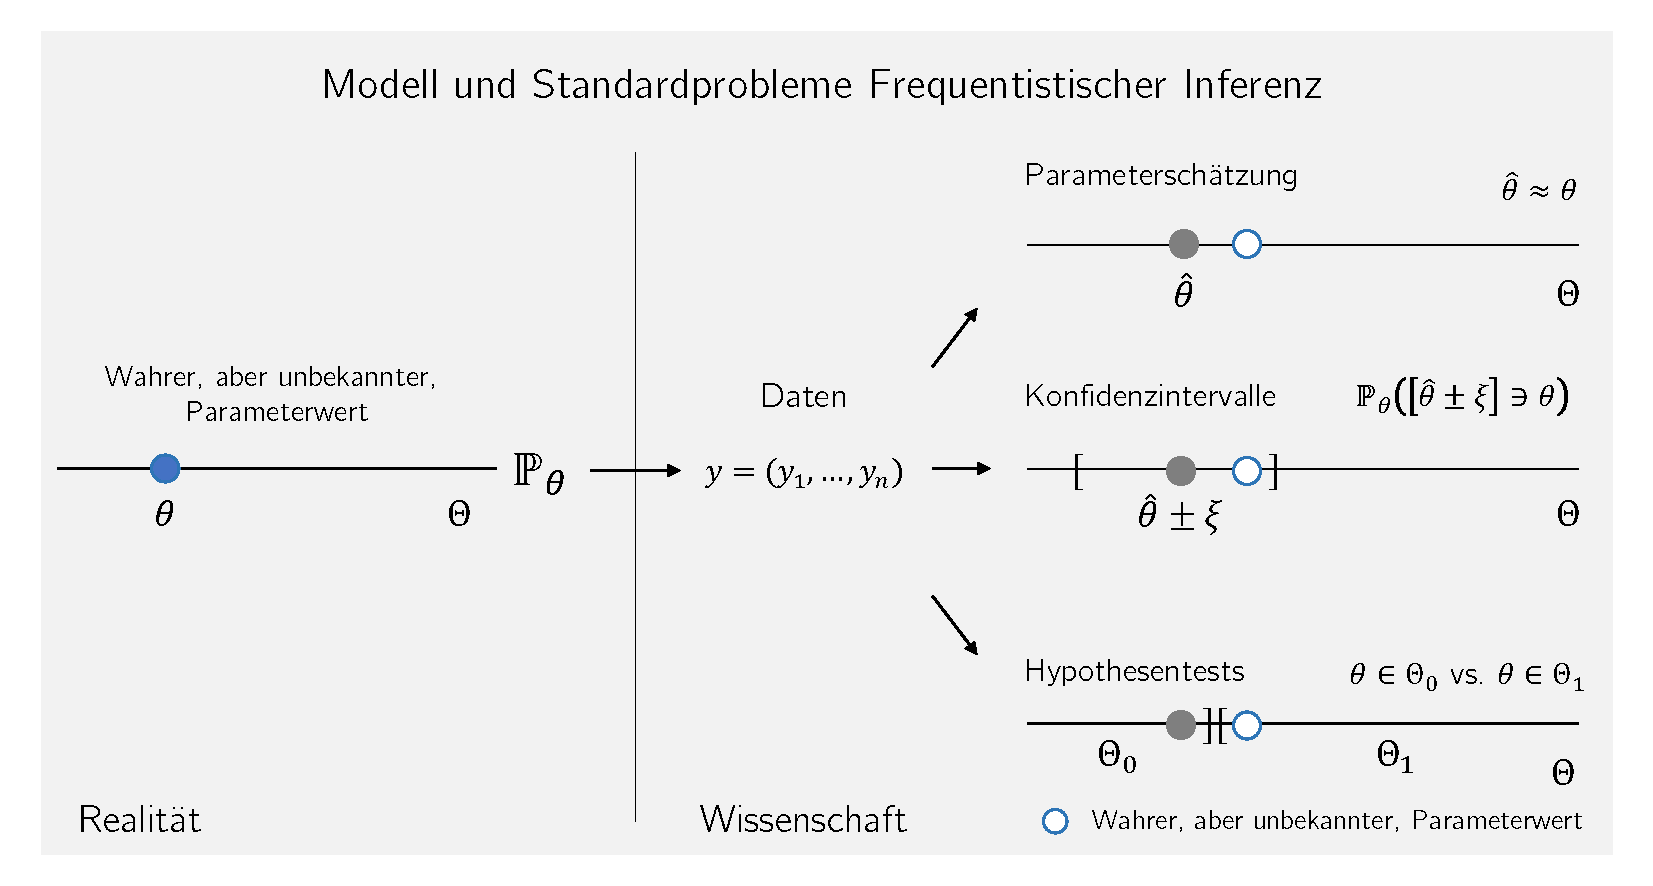
\includegraphics[width=1\linewidth]{12_Abbildungen/wtfi_12_frequentistische_inferenz} \end{center}
\end{frame}

\begin{frame}{}
\protect\hypertarget{section-3}{}
\begin{center}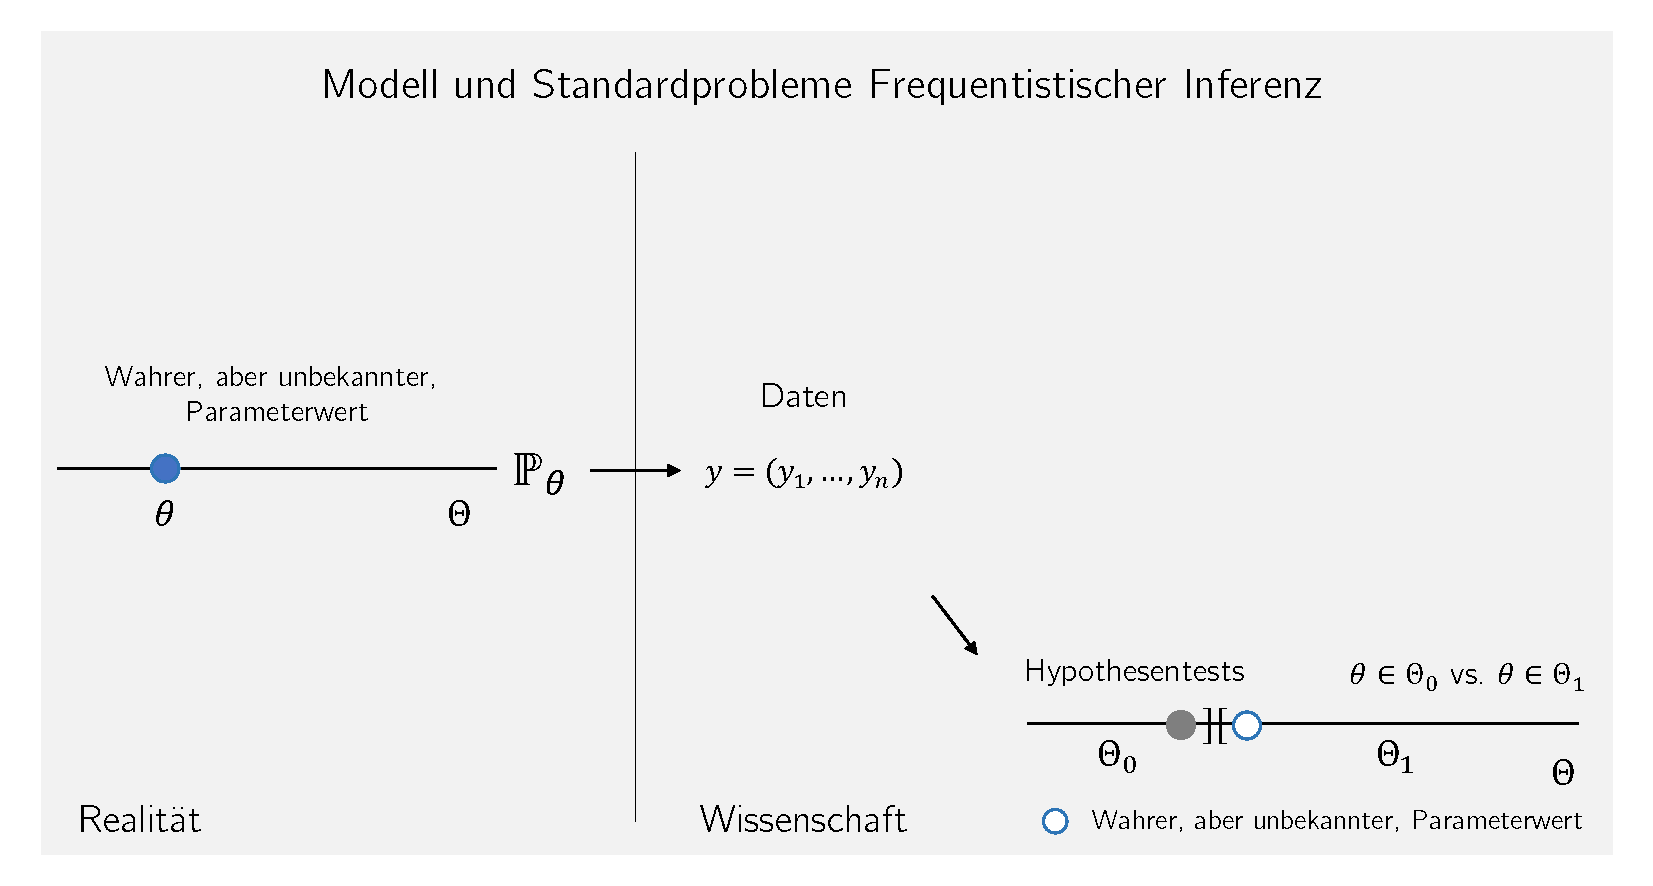
\includegraphics[width=1\linewidth]{12_Abbildungen/wtfi_12_frequentistische_inferenz_hypothesentests} \end{center}
\end{frame}

\begin{frame}{}
\protect\hypertarget{section-4}{}
\textcolor{darkblue}{Standardannahmen Frequentistischer Inferenz}

\footnotesize

\(\mathcal{M}\) sei ein statistisches Modell mit Stichprobe
\(\ups_1,...,\ups_n \sim p_\theta\). \textbf{Es wird angenommen, dass
ein konkret vorliegender Datensatz
\(y = (y_1,...,y_n) \in \mathbb{R}^n\) eine der möglichen Realisierungen
von \(\ups_1,...,\ups_n \sim p_\theta\) ist.} Aus Frequentistischer
Sicht kann man eine Studie unter gleichen Umständen unendlich oft
wiederholen und zu jedem Datensatz Schätzer oder Statistiken auswerten,
z.B. das Stichprobenmittel:

\footnotesize
\begin{itemize}
\item[] Datensatz (1) : $y^{(1)} = \left(y_1^{(1)}, y_2^{(1)}, ...,y_n^{(1)}\right)$
                        mit $\bar{y}_n^{(1)} = \frac{1}{n}\sum_{i=1}^n y_i^{(1)}$
\item[] Datensatz (2) : $y^{(2)} = \left(y_1^{(2)}, y_2^{(2)}, ...,y_n^{(2)}\right)$
                        mit $\bar{y}_n^{(2)} = \frac{1}{n}\sum_{i=1}^n y_i^{(2)}$
\item[] Datensatz (3) : $y^{(3)} = \left(y_1^{(3)}, y_2^{(3)}, ...,y_n^{(3)}\right)$
                        mit $\bar{y}_n^{(3)} = \frac{1}{n}\sum_{i=1}^n y_i^{(3)}$
\item[] Datensatz (4) : $y^{(4)} = \left(y_1^{(4)}, y_2^{(4)}, ...,y_n^{(4)}\right)$
                        mit $\bar{y}_n^{(4)} = \frac{1}{n}\sum_{i=1}^n y_i^{(4)}$
\item[] Datensatz (5) : $y^{(5)} = ...$
\end{itemize}

Um die Qualität statistischer Methoden zu beurteilen betrachtet die
Frequentistische Statistik deshalb die Wahrscheinlichkeitsverteilungen
von Schätzern und Statistiken unter Annahme von
\(\ups_1,...,\ups_n \sim p_\theta\). Was zum Beispiel ist die Verteilung
der \(\bar{y}_n^{(1)}\), \(\bar{y}_n^{(2)}\), \(\bar{y}_n^{(3)}\),
\(\bar{y}_n^{(4)}\), \ldots{} also die Verteilung der Zufallsvariable
\(\bar{\ups}\)?

Wenn eine statistische Methode im Sinne der Frequentistischen
Standardannahmen ``gut'' ist, dann heißt das also, dass sie bei häufiger
Anwendung ``im Mittel gut'' ist. Im Einzelfall, also im Normalfall nur
eines vorliegenden Datensatzes, kann sie auch ``schlecht'' sein.
\end{frame}

\begin{frame}{}
\protect\hypertarget{section-5}{}
\textcolor{darkblue}{Grundlegende Logik Frequentistischer Hypothesentests}

\footnotesize

\justifying Man hat einen Datensatz \(y_1,...,y_n\) vorliegen und nimmt
an, dass es sich dabei um die Realisation einer Stichprobe handelt, zum
Beispiel von \(\ups_1,...,\ups_n \sim N(\mu,\sigma^2)\).

Man berechnet basierend auf dem Datensatz eine \emph{Teststatistik}, zum
Beispiel das anhand der Stichprobenvarianz und der Stichprobengröße
normalisierte Stichprobenmittel \(\sqrt{n}\bar{y}_n/s_n\).

Man fragt sich, wie wahrscheinlich es wäre, den beobachteten oder einen
extremeren Wert der Teststatistik unter der Annahme eines
\emph{Nullmodels} zu observieren. Dabei meint man mit \emph{Nullmodell}
intuitiv ein Wahrscheinlichkeitsverteilungsmodell bei dem kein
``interessanter Effekt'' vorliegt, also zum Beispiel \(\mu = 0\) gilt.
Die Wahrscheinlichkeit ist wie immer Frequentistisch zu verstehen, d.h.
als idealisierte relative Häufigkeit, wenn man viele
Stichprobenrealisationen des Nullmodels generieren würde.

Ist die betrachtete Wahrscheinlichkeit dafür, den beobachteten oder
einen extremeren Wert der Teststatistik unter Annahme des Nullmodells zu
observieren groß, so sagt man sich ``Nunja, dann ist es wohl ganz
plausibel, dass das Nullmodel die Daten generiert hat''. Im
Wissenschaftsjargon spricht man von einem ``nicht-signifikanten
Ergebnis''.

Ist die betrachtete Wahrscheinlichkeit dafür, den beobachteten oder
einen extremeren Wert der Teststatistik unter Annahme des Nullmodells zu
observieren dagegen klein, so sagt man sich ``Aha, dann ist es wohl
nicht so plausibel, dass das Nullmodel die Daten generiert hat''. Im
Wissenschaftsjargon spricht man von einem ``signifikanten Ergebnis''.

Wie immer in der Frequentistischen Statistik weiß man nach Durchführung
dieser Prozedur nicht, ob im vorliegenden Fall nun wirklich das
Nullmodel oder ein anderes Modell die Daten generiert hat, sondern man
weiß nur, wie oft man bei dieser Prozedur im Mittel richtig oder falsch
liegen würde, wenn alle Annahmen zuträfen und man diese Prozedur sehr
oft wiederholen würde.
\end{frame}

\begin{frame}{}
\protect\hypertarget{section-6}{}
\setstretch{2.4}
\large
\vfill

Grundlegende Definitionen

Einstichproben-T-Test

p-Werte

Konfidenzintervalle und Hypothesentests

Anwendungsbeispiel

Selbstkontrollfragen \vfill
\end{frame}

\begin{frame}{}
\protect\hypertarget{section-7}{}
\setstretch{2.4}
\large
\vfill

\textbf{Grundlegende Definitionen}

Einstichproben-T-Test

p-Werte

Konfidenzintervalle und Hypothesentests

Anwendungsbeispiel

Selbstkontrollfragen \vfill
\end{frame}

\begin{frame}{Grundlegende Definitionen}
\protect\hypertarget{grundlegende-definitionen}{}
\small
\begin{definition}[Statistische Hypothesen und Testszenario]
\justifying
$\ups_1,...,\ups_n \sim p_\theta$ sei eine Stichprobe mit WMF oder WDF $p_\theta$,
$\mathcal{Y}$ sei der Ergebnisraum des Zufallsvektors $\ups := (\ups_1,...,\ups_n)$, und
$\Theta$ sei der Parameterraum des zugrundeliegenden statistischen Modells.
Weiterhin sei $\{\Theta_0,\Theta_1\}$ eine Partition des Parameterraumes, so
dass $\Theta = \Theta_0 \cup \Theta_1$ und $\Theta_0 \cap \Theta_1 = \emptyset$
gelten. Eine \textit{statistische Hypothese} ist dann eine Aussage über den
wahren, aber unbekannten, Parameterwert $\theta$ in Hinblick auf die Untermengen
$\Theta_0$ und $\Theta_1$ des Parameterraums. Speziell werden die Aussagen
\begin{itemize}
\item $\theta \in \Theta_0$ als \textit{Nullhypothese} $H_0$
\item $\theta \in \Theta_1$ als \textit{Alternativhypothese} $H_1$
\end{itemize}
bezeichnet. Die Einheit aus Stichprobe, Ergebnisraum, Parameterraum, und
Hypothesen wird im Folgenden als \textit{Testszenario} bezeichnet.
\end{definition}
\end{frame}

\begin{frame}{Grundlegende Definitionen}
\protect\hypertarget{grundlegende-definitionen-1}{}
\small
\begin{definition}[Einfache und zusammengesetzte Hypothesen]
\justifying
Für statistische Hypothesen $\Theta_i,i = 0,1$ gilt:
\begin{itemize}
\item Enthält $\Theta_i$ nur ein einziges Element, so heißt $\Theta_i$ \textit{einfach}.
\item Enthält $\Theta_i$ mehr als ein Element, so heißt $\Theta_i$ \textit{zusammengesetzt}.
\end{itemize}
\end{definition}

Bemerkungen

\begin{itemize}
\tightlist
\item
  Die Nullhypothese \(\Theta_0 = \{0\}\) ist ein Beispiel für eine
  einfache Hypothese.
\item
  Bei einer einfachen Hypothese ist die Wahrscheinlichkeitsverteilung
  von \(\ups\) genau festgelegt.
\item
  Bei einer zusammengesetzten Hypothese ist nur die Verteilungsklasse
  von \(\ups\) festgelegt.
\end{itemize}
\end{frame}

\begin{frame}{Grundlegende Definitionen}
\protect\hypertarget{grundlegende-definitionen-2}{}
\small
\setstretch{1.2}

\begin{definition}[Einseitige und zweiseitige Hypothesen]
\justifying
$\Theta := \mathbb{R}$ sei ein eindimensionaler Parameterraum und $\theta_0$
sei ein Element von $\Theta$. Dann werden zusammengesetzte Nullhypothesen der
Form
\begin{equation}
\Theta_0 := ]-\infty,\theta_0] \mbox{ oder }
\Theta_0 := [\theta_0,\infty[
\end{equation}
\textit{einseitige Nullhypothesen} genannt und auch in der Form
\begin{equation}
H_0 : \theta \le \theta_0 \mbox{ oder } H_0 : \theta \ge \theta_0
\end{equation}
geschrieben. Die entsprechenden Alternativhypothesen haben dabei die Form
\begin{equation}
\Theta_1 := ]\theta_0,\infty[ \mbox{ oder } \Theta_1 := ]-\infty, \theta_0[
\mbox{ bzw. }  H_1 : \theta > \theta_0 \mbox{ oder } H_1 : \theta < \theta_0.
\end{equation}
Bei einer einfachen Nullhypothese der Form
\begin{equation}
\Theta_0 := \{\theta_0\} \mbox{ bzw. } H_0 : \theta = \theta_0
\end{equation}
wird die Alternativhypothese
\begin{equation}
\Theta_1 := \Theta \setminus \{\theta_0\} \mbox{ bzw. } H_1 : \theta \neq \theta_0
\Leftrightarrow \Theta_1 := ]-\infty, \theta_0[\,\, \cup \,\,]\theta_0,\infty[
\end{equation}
\textit{zweiseitige Alternativhypothese} genannt.
\end{definition}
\end{frame}

\begin{frame}{Grundlegende Definitionen}
\protect\hypertarget{grundlegende-definitionen-3}{}
\small
\begin{definition}[Test]
\justifying
In einem Testszenario ist ein \textit{Test} $\phi$ eine Abbildung aus dem
Ergebnisraum $\mathcal{Y}$ nach $\{0,1\}$,
\begin{equation}
\phi : \mathcal{Y} \to \{0,1\}, y \mapsto \phi(y).
\end{equation}
Dabei repräsentiert
\begin{itemize}
\item $\phi(y) = 0$ den Vorgang des Nichtablehnens der Nullhypothese.
\item $\phi(y) = 1$ den Vorgang des Ablehnens der Nullhypothese.
\end{itemize}
\end{definition}

\footnotesize

Bemerkung

\begin{itemize}
\tightlist
\item
  Weil \(y\) eine Realisation von \(\ups\) ist, ist \(\phi(y)\) eine
  Realisation von \(\phi(\ups)\).
\end{itemize}
\end{frame}

\begin{frame}{Grundlegende Definitionen}
\protect\hypertarget{grundlegende-definitionen-4}{}
\small
\begin{definition}[Standardtest]
\justifying
Ein \textit{Standardtest} ist definiert durch die Verkettung einer
\textit{Teststatistik}
\begin{equation}
\gamma : \mathcal{Y} \to \mathbb{R}
\end{equation}
und einer \textit{Entscheidungsregel}
\begin{equation}
\delta : \mathbb{R} \to \{0,1\}.
\end{equation}
Ein Standardtest kann also geschrieben werden als
\begin{equation}
\phi := \delta \circ \gamma : \mathcal{Y} \to \{0,1\}.
\end{equation}
\end{definition}

\footnotesize

Bemerkungen

\begin{itemize}
\tightlist
\item
  Weil \(y\) eine Realisation von \(\ups\) ist, ist
  \(\gamma(y) \in \mathbb{R}\) eine Realisation von \(\gamma(\ups)\).
\item
  Weil \(\gamma(y)\) eine Realisation von \(\gamma(\ups)\) ist, ist
  \((\delta \circ \gamma)(y)\) eine Realisation von
  \((\delta \circ \gamma)(\ups)\).
\item
  Wir betrachten in der Folge nur Standardtests.
\end{itemize}
\end{frame}

\begin{frame}{Grundlegende Definitionen}
\protect\hypertarget{grundlegende-definitionen-5}{}
\small
\begin{definition}[Kritischer Bereich]
\justifying
Die Untermenge $K$ des Ergebnisraums des Zufallsvektors $\ups := (\ups_1,...,\ups_n)$,
für die ein Test den Wert 1 annimmt, heißt \textit{kritischer Bereich} des Tests,
\begin{equation}
K := \{y \in \mathcal{Y} |\phi(y) = 1 \} \subset \mathcal{Y}.
\end{equation}
\end{definition}

Bemerkungen

\begin{itemize}
\tightlist
\item
  Die Ereignisse \(\{\phi(\ups) = 1\}\) und \(\{\ups\in K\}\) sind
  äquivalent.
\item
  Die Ereignisse \(\{\phi(\ups) = 1\}\) und \(\{\ups\in K\}\) haben die
  gleiche Wahrscheinlichkeit.
\end{itemize}
\end{frame}

\begin{frame}{Grundlegende Definitionen}
\protect\hypertarget{grundlegende-definitionen-6}{}
\small
\begin{definition}[Ablehnungsbereich]
\justifying
Die Untermenge $A$ des Ergebnisraums einer Teststatistik, für die der Test
den Wert 1 annimmt, heißt \textit{Ablehnungsbereich} des Tests,
\begin{equation}
A := \{\gamma(y) \in \mathbb{R} |\phi(y) = 1 \} \subset \mathbb{R}.
\end{equation}
\end{definition}

Bemerkungen

\begin{itemize}
\tightlist
\item
  Die Ereignisse \(\{\phi(\ups) = 1\}\) und \(\{\gamma(\ups) \in A\}\)
  sind äquivalent.
\item
  Die Ereignisse \(\{\phi(\ups) = 1\}\) und \(\{\gamma(\ups) \in A\}\)
  haben die gleiche Wahrscheinlichkeit.
\end{itemize}
\end{frame}

\begin{frame}{Grundlegende Definitionen}
\protect\hypertarget{grundlegende-definitionen-7}{}
\small
\begin{definition}[Kritischer Wert-basierte Tests]
\justifying
Ein \textit{kritischer Wert-basierter Test} ist ein Standardtest, bei dem die
Entscheidungsregel $\delta$ von einem kritischen Wert $k \in \mathbb{R}$ abhängt.
Speziell ist
\begin{itemize}
\item ein \textit{einseitiger kritischer Wert-basierter Test} von der Form
\begin{equation}
\phi : \mathcal{Y} \to \{0,1\}, y \mapsto \phi(y) := 1_{\{\gamma(y) \ge k\}} =
\begin{cases}
1 & \gamma(y) \ge k \\
0 & \gamma(y) < k
\end{cases}
\end{equation}
\item ein \textit{zweiseitiger kritischer Wert-basierter Test} von der Form
\begin{equation}
\phi : \mathcal{Y} \to \{0,1\}, y \mapsto \phi(y) := 1_{\{|\gamma(y)| \ge k\}} =
\begin{cases}
1 & |\gamma(y)| \ge k \\
0 & |\gamma(y)| < k
\end{cases}
\end{equation}
\end{itemize}
\end{definition}

Bemerkung

\begin{itemize}
\tightlist
\item
  Wir betrachten in der Folge nur kritischer Wert-basierte Tests.
\end{itemize}
\end{frame}

\begin{frame}{Grundlegende Definitionen}
\protect\hypertarget{grundlegende-definitionen-8}{}
\small
\begin{definition}[Richtige Testentscheidungen und Testfehler]
\justifying
Das Nichtablehnen der Nullhypothese, wenn die Nullhypothese zutrifft werden,
sowie das Ablehnen der Nullhypothese, wenn die Nullhypothese nicht zutrifft,
werden \textit{richtige Testentscheidungen} genannt. Es können weiterhin zwei
Arten von Testfehlern auftreten: das Ablehnen der Nullhypothese, wenn die
Nullhypothese zutrifft, heißt \textit{Typ I Fehler}, das Nichtablehnen der
Nullhypothese, wenn die Alternativhypothese zutrifft, heißt
\textit{Typ II Fehler}.
\end{definition}

Die untenstehende Graphik gibt eine Übersicht. \vspace{1mm}

\begin{center}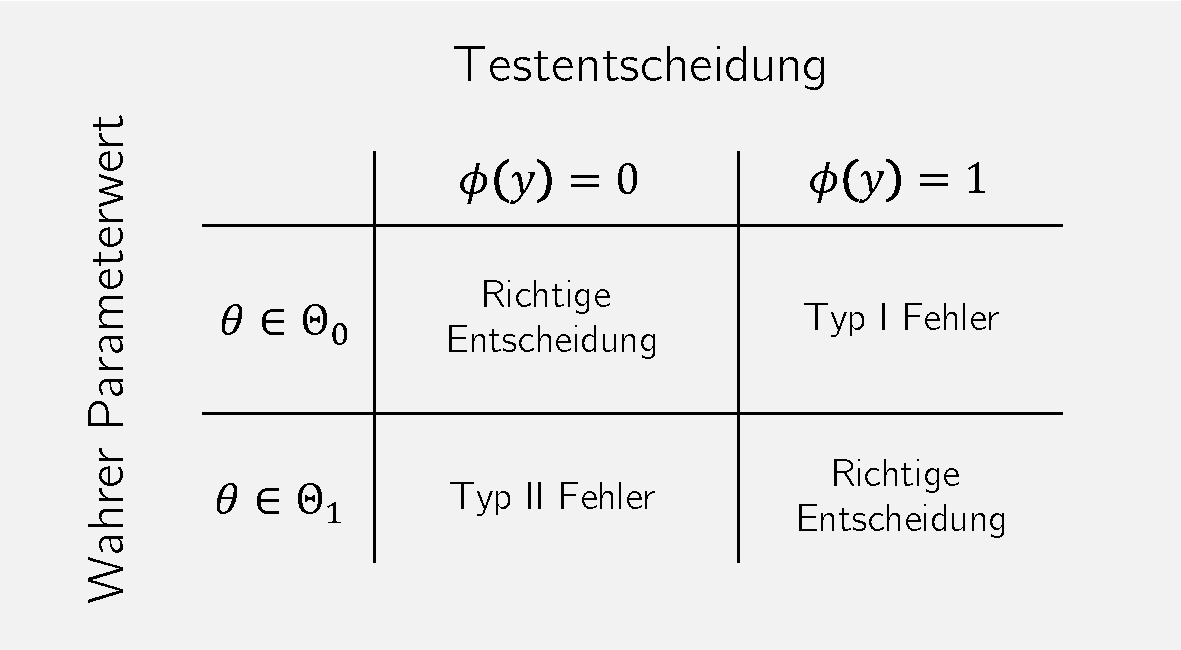
\includegraphics[width=0.55\linewidth]{12_Abbildungen/wtfi_12_testfehler} \end{center}
\end{frame}

\begin{frame}{Grundlegende Definitionen}
\protect\hypertarget{grundlegende-definitionen-9}{}
\small
\begin{definition}[Testgütefunktion]
\justifying
Für einen Test $\phi$ ist die \textit{Testgütefunktion} definiert als
\begin{equation}
q_{\phi} : \Theta \to [0,1], \theta \mapsto q_{\phi}(\theta) := \mathbb{P}_\theta(\phi = 1).
\end{equation}
Für $\theta \in \Theta_1$ heißt $q_\phi$ auch \textit{Powerfunktion} oder
\textit{Trennschärfefunktion}.
\end{definition}
\footnotesize

Bemerkungen

\begin{itemize}
\tightlist
\item
  Wir verzichten hier und im Folgenden auf die explizite Notation der
  Abhängigkeit von \(\phi\) von \(\ups\).
\item
  \(\mathbb{P}_\theta\) bezeichnet die Verteilung von \(\phi\) unter der
  Annahme \(\ups_1,...,\ups_n \sim p_\theta\).
\item
  Es gilt
  \(\mathbb{P}_\theta(\phi = 1) = \mathbb{P}_\theta (\ups \in K) = \mathbb{P}_\theta(\gamma \in A)\)
\item
  Für jedes \(\theta \in \Theta\) liefert \(q_\phi\) die
  Wahrscheinlichkeit, dass \(H_0\) durch \(\phi\) abgelehnt wird.
\item
  Bei Poweranalysen betrachtet man \(q_{\phi}\) als Funktion aller
  Testszenario und Testparameter.
\item
  Ändert sich \(\phi\), z.B. weil sich der kritische Wert von \(\phi\)
  ändert, dann ändert sich \(q_{\phi}(\theta)\).
\item
  Im Idealfall hätte man einen Test \(\phi\) mit \begin{equation}
  q_\phi(\theta) = \mathbb{P}_\theta(\phi = 1) = 0 \mbox{ für } \theta \in \Theta_0 \mbox{ und }
  q_\phi(\theta) = \mathbb{P}_\theta(\phi = 1) = 1 \mbox{ für } \theta \in \Theta_1.
  \end{equation}
\item
  Die Testentscheidung eines solchen \(\phi\) wäre mit
  Wahrscheinlichkeit 1 richtig.
\end{itemize}
\end{frame}

\begin{frame}{Grundlegende Definitionen}
\protect\hypertarget{grundlegende-definitionen-10}{}
\textcolor{darkblue}{Intuition zur Testkonstruktion} \small

Im Idealfall hätte man einen Test \(\phi\) mit \begin{equation}
q_\phi(\theta) = \mathbb{P}_\theta(\phi = 1) = 0 \mbox{ für } \theta \in \Theta_0 \mbox{ und }
q_\phi(\theta) = \mathbb{P}_\theta(\phi = 1) = 1 \mbox{ für } \theta \in \Theta_1.
\end{equation}

\(\Rightarrow\) Gut sind kleine Werte von \(q_\phi\) für
\(\theta \in \Theta_0\) und große Werte von \(q_\phi\) für
\(\theta \in \Theta_1\).

Generell gibt es Abhängigkeiten zwischen den Werten von \(q_\phi\) für
\(\theta \in \Theta_0\) und \(\theta \in \Theta_1\):

\footnotesize

Sei zum Beispiel \(\phi_a\) der Test definiert durch \(\phi_a(y) := 0\)
für alle \(y \in \mathcal{Y}\), also der Test, der die Nullhypothese,
unabhängig von den beobachteten Daten, \textit{niemals ablehnt}. Für
diesen Test gilt \(q_{\phi_a}(\theta) = 0\) für \(\theta \in \Theta_0\).
Allerdings gilt für diesen Test auch \(q_{\phi_a}(\theta) = 0\) für
\(\theta \in \Theta_1\).

Andersherum sei \(\phi_b\) der Test definiert durch \(\phi_b(y) := 1\)
für alle \(y \in \mathcal{Y}\), also ein Test, der die Nullhypothese,
unabhängig von den beobachteten Daten, \textit{immer ablehnt}. Für
diesen Test gilt \(q_{\phi_b}(\theta) = 1\) für \(\theta \in \Theta_1\).
Allerdings gilt für diesen Test auch \(q_{\phi_b}(\theta) = 1\) für
\(\theta \in \Theta_0\).

\small

In der Konstruktion eines Tests muss also eine angemessene Balance
zwischen kleinen Werten von \(q_\phi\) für \(\theta \in \Theta_0\) und
großen Werten von \(q_\phi\) für \(\theta \in \Theta_1\) gefunden
werden.
\end{frame}

\begin{frame}{Grundlegende Definitionen}
\protect\hypertarget{grundlegende-definitionen-11}{}
\textcolor{darkblue}{Intuition zur Testkonstruktion} \small

Die populärste Methode, eine Balance zwischen zwischen kleinen Werten
von \(q\) für \(\theta \in \Theta_0\) und großen Werten von \(q\) für
\(\theta \in \Theta_1\) zu finden, ist in einem ersten Schritt ein
\(\alpha_0 \in [0,1]\) zu wählen und sicher zu stellen, dass
\begin{equation}\label{eq:significance}
q_\phi(\theta) \le \alpha_0 \mbox{ für alle } \theta \in \Theta_0.
\end{equation}

Eine konventionelle Wahl für sein solches \(\alpha_0\) ist zum Beispiel
\(\alpha_0 := 0.05\).

Unter allen Tests und statistischen Modellen, die Ungleichung
\eqref{eq:significance} erfüllen, wird man dann einen Test oder ein
statistisches Modell auswählen, so dass \(q_\phi(\theta)\) für
\(\theta \in \Theta_1\) so groß wie möglich ist.

Dieses Vorgehen ist nicht alternativlos, man kann zum Beispiel auch
lineare Kombinationen verschiedener Fehlerwahrscheinlichkeiten
minimieren. Es ist aber das in der Anwendung populärste Vorgehen. Wir
werden uns deshalb in der Folge auf dieses Vorgehen beschränken.

Das beschriebene Vorgehen motiviert die folgenden Definitionen der
Begriffe des Level-\(\alpha_0\)-Tests, des Signifikanzlevels
\(\alpha_0\) (oft auch als \emph{Signifikanzlevel} bezeichnet) und des
Testumfangs \(\alpha\) (auch als \emph{effektives Niveau} bezeichnet).
\end{frame}

\begin{frame}{Grundlegende Definitionen}
\protect\hypertarget{grundlegende-definitionen-12}{}
\small
\begin{definition}[Level-$\alpha_0$-Test, Signifikanzlevel $\alpha_0$,
Testumfang $\alpha$]
$q_\phi$ sei die Testgütefunktion eines Tests $\phi$ und es sei
$\alpha_0 \in [0,1]$. Dann heißt ein Test $\phi$, für den gilt, dass
\begin{equation}
q_\phi(\theta) \le \alpha_0 \mbox{ für alle } \theta \in \Theta_0
\end{equation}
ein \textit{Level-$\alpha_0$-Test} und man sagt, dass der Test das
\textit{Signifikanzlevel $\alpha_0$} hat. Die Zahl
\begin{equation}
\alpha := \max_{\theta \in \Theta_0} q_\phi(\theta) \in [0,1]
\end{equation}
heißt der \textit{Testumfang} von $\phi$.
\end{definition}

Bemerkungen

\begin{itemize}
\tightlist
\item
  \(\alpha\) ist die größtmögliche Wahrscheinlichkeit für einen Typ I
  Fehler.
\item
  Ein Test ist dann, und nur dann, ein Level-\(\alpha_0\)-Test, wenn
  \(\alpha \le \alpha_0\) gilt.
\item
  Bei einer einfachen Nullhypothese gilt für den Testumfang, dass
  \(\alpha = q_{\phi}(\theta_0) = \mathbb{P}_{\theta_0}(\phi = 1)\).
\end{itemize}
\end{frame}

\begin{frame}{Grundlegende Definitionen}
\protect\hypertarget{grundlegende-definitionen-13}{}
\textcolor{darkblue}{Typ I Fehlerwahrscheinlichkeit vs. Testumfang vs. Signifikanzlevel}

\small

Bei einfacher \(\Theta_0\) ist der Testumfang gleich der
Wahrscheinlichkeit eines Typ I Fehlers \begin{equation}
\alpha
:= \max_{\theta \in \Theta_0} q_\phi(\theta)
=  \max_{\theta \in \{\theta_0\}} q_\phi(\theta)
= q_\phi(\theta_0)
= \mathbb{P}_{\theta_0}(\phi = 1).
\end{equation}

Bei zusammengesetzter \(\Theta_0\) gibt es je nach Wert von
\(\theta \in \Theta_0\) verschiedene Wahrscheinlichkeiten für einen Typ
I Fehler. Die größte dieser Wahrscheinlichkeiten ist der Testumfang
\begin{equation}
\alpha
:= \max_{\theta \in \Theta_0} q_\phi(\theta)
 = \max_{\theta \in \Theta_0} \mathbb{P}_{\theta}(\phi = 1).
\end{equation}

Ein Test hat Signifikanzlevel \(\alpha_0\), wenn der Testumfang kleiner
oder gleich \(\alpha_0\) ist. \begin{equation}
\alpha
=   \max_{\theta \in \Theta_0} q_\phi(\theta)
\le \alpha_0
\end{equation}

Ein Test, bei dem das Signifikanzlevel größer als der Testumfang ist,
heißt \emph{konsvervativ}.

Ein Test, bei dem das Signifikanzlevel gleich dem Testumfang ist, heißt
\emph{exakt}.
\end{frame}

\begin{frame}{Grundlegende Definitionen}
\protect\hypertarget{grundlegende-definitionen-14}{}
\textcolor{darkblue}{Zur Wahl von Nullhypothese und Alternativhypothese}

\small

Das Vorgehen in der Testkonstruktion zunächst durch die Wahl eines
Signifikanzlevels den Testumfang zu begrenzen und erst in einem zweiten
Schritt dafür zu sorgen, dass die Wahrscheinlichkeit von \(\phi = 1\)
bei \(\theta \in \Theta_1\) bei diesem Signifikanzlevel möglichst groß
ist, induziert eine Asymmetrie in der Behandlung von Null- und
Alternativhypothese. Implizit wichtet man mit diesem Vorgehen Typ I
Fehler als schwerwiegender als Typ II Fehler.

Dies wiederum impliziert eine mögliche Strategie zur Festlegung von
Null- und Alternativhypothese: Die Nullhypothese ist die Hypothese,
hinsichtlich deren assoziierter Testentscheidung man eher keinen Fehler
machen möchte bzw. deren Fehlerwahrscheinlichkeit man primär
kontrollieren möchte.

In der wissenschaftichen Anwendung ist es Standard, die falsche
Konfirmation der eigenen Theorie als einen schwerwiegenderen Fehler als
die falsche Ablehnung der eigenen Theorie zu werten.

Die falsche Konfirmation der eigenen Theorie sollte also ein Typ I
Fehler, das falsche Ablehnen der eigenen Theorie ein Typ II Fehler sein.

Damit die falsche Konfirmation der eigenen Theorie einen Typ I Fehler,
also das Ablehnen von \(H_0\) bei Zutreffen von \(H_0\), darstellt, muss
die eigene Theorie als Alternativhypothese aufgestellt werden. Die
Alternativhypothese fälschlichweise Abzulehnen wird damit ein Typ II
Fehler.
\end{frame}

\begin{frame}{Grundlegende Definitionen}
\protect\hypertarget{grundlegende-definitionen-15}{}
\textcolor{darkblue}{Kommentar zum Frequentistischen Hypothesentesten in der Wissenschaft}

\small

Frequentistisches Hypothesentesten ist als Entscheidungsproblem ohne
klar und explizit definierte Entscheidungsnutzenfunktion formuliert und
deshalb recht mühselig zu analysieren und zu studieren. Es gibt sehr
viel zugänglichere Theorien zu Entscheidungen unter Unsicherheit (vgl.
Pratt, Raiffa, and Schlaifer (1995), Puterman (2005), Ostwald, Starke,
and Hertwig (2015), Horvath et al. (2021))

Oberflächlich betrachtet liefern Hypothesentests einfache binäre
Aussagen der Form ``Die Hypothese (Theorie) ist gegeben die Evidenz
abzulehnen oder zu akzeptieren''. Solche Aussagen sind im
Entscheidungskontext hilfreich, denn es muss etwas passieren, also eine
Entscheidung getroffen werden. In der Wissenschaft, also der
menschlichen Kommunikationsstruktur über die Beschaffenheit der Welt,
muss aber nichts final entschieden, sondern nur das Maß an Unsicherheit
über den gerade vorherrschenden Theoriestand quantifiziert und
kommuniziert werden. Generell sollten Fragestellungen der
Grundlagenwissenschaften deshalb gerade nicht als Entscheidungsprobleme
formuliert werden.

Trotz landläufiger Meinung das Bayesianische Herangehensweisen wie
Positive Predictive Values oder Bayes Factors hier irgendwie besser
sind, ist dem nicht so, so lange die mit einer gewissen Modellpräferenz
assoziierte Unsicherheit nicht klar mitkommuniziert wird.

Und trotz alledem ist Frequentistisches Hypothesentesten in der
Wissenschaftscommunity weiterhin sehr populär (wenn auch vermutlich
nicht immer ganz verstanden) und sollte deshalb im Rahmen eines
wissenschaftlichen Studiums wie der Psychologie intellektuell
durchdrungen werden.
\end{frame}

\begin{frame}{}
\protect\hypertarget{section-8}{}
\setstretch{2.4}
\large
\vfill

Grundlegende Definitionen

\textbf{Einstichproben-T-Test}

p-Werte

Konfidenzintervalle und Hypothesentests

Anwendungsbeispiel

Selbstkontrollfragen \vfill
\end{frame}

\begin{frame}{Einstichproben-T-Test}
\protect\hypertarget{einstichproben-t-test}{}
Beispiel \textbar{} Evidenzbasierte Evaluation von Psychotherapie bei
Depression

\begin{center}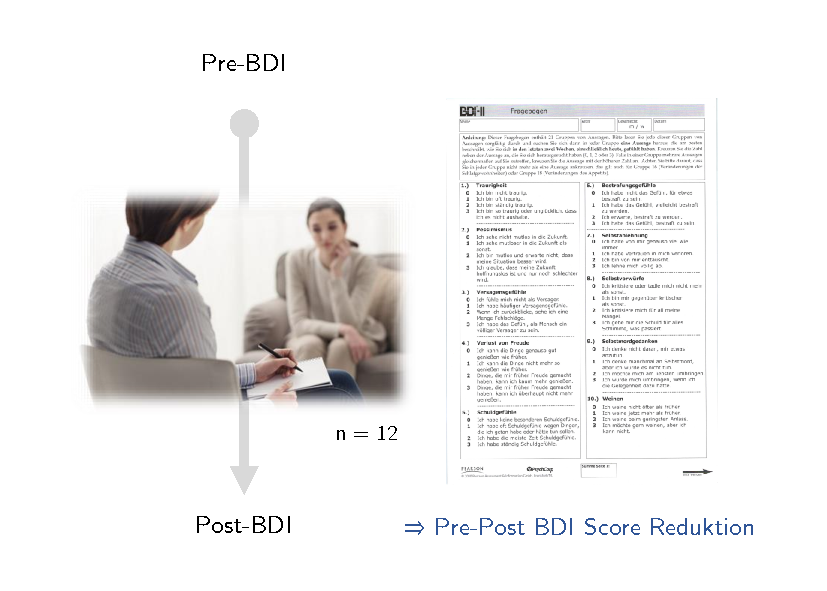
\includegraphics[width=0.8\linewidth]{12_Abbildungen/wtfi_12_messplan} \end{center}
\end{frame}

\begin{frame}{Einstichproben-T-Test}
\protect\hypertarget{einstichproben-t-test-1}{}
Beispiel \textbar{} Evidenzbasierte Evaluation von Psychotherapie bei
Depression \vspace{2mm}

\small

Für die Pre-Post BDI Score Reduktion \(\ups_i\) der \(i\)ten von \(n\)
Patient:innen legen wir das Modell \begin{equation}
\ups_{i} = \mu + \varepsilon_{i} \mbox{ mit } \varepsilon_{i} \sim N(0,\sigma^2) \mbox{ u.i.v. für } i = 1,...,n
\end{equation} zugrunde. Dabei wird die Pre-Post BDI Reduktion
\(\ups_i\) der \(i\)ten Patient:in also mithilfe einer über die Gruppe
von Patient:innen identischen Pre-Post BDI Score Reduktion
\(\mu \in \mathbb{R}\) und einer Patient:innen-spezifischen
normalverteilten Pre-Post BDI Score Reduktionsabweichung
\(\varepsilon_{i}\) erklärt

Wie gezeigt ist dieses Modell äquivalent zum Normalverteilungsmodell
\begin{equation}
\ups_1,...,\ups_n \sim N(\mu,\sigma^2).
\end{equation}

\(\Rightarrow\) Wir seien nun am Testen einer statistischen Hypothese
hinsichtlich \(\mu\) interessiert.

\(\Rightarrow\) Das betrachtete Anwendungsszenario ist dann ein Beispiel
für einen \textbf{Eintstichproben-T-Test}.
\end{frame}

\begin{frame}{Einstichproben-T-Test}
\protect\hypertarget{einstichproben-t-test-2}{}
Mögliche Hypothesen im Einstichproben-Test-Szenario \small
\setstretch{1.1}

Einfache Nullhypothese, einfache Alternativhypothese
\(H_0:\mu = \mu_0, H_1:\mu = \mu_1\)

\begin{itemize}
\item Theoretisch wichtiges Szenario (Neymann-Pearson Lemma)
\item Praktische Relevanz eher gering
\end{itemize}

Einfache Nullhypothese, zusammengesetzte Alternativhypothese
\(H_0:\mu = \mu_0, H_1:\mu \neq \mu_0\)

\begin{itemize}
\item Zweiseitiger Einstichproben-T-Test mit ungerichteter Hypothese
\item Ungerichtete Fragestellung nach einem Unterschied
\end{itemize}

Zusammengesetzte Nullhypothese/Alternativhypothese
\(H_0:\mu \le \mu_0, H_1:\mu > \mu_0\)

\begin{itemize}
\item Einseitiger Einstichproben-T-Test mit gerichteter Hypothese
\item Gerichtete Fragestellung nach einem positiven Unterschied
\end{itemize}

Zusammengesetzte Nullhypothese/Alternativhypothese
\(H_0:\mu\ge\mu_0,H_1:\mu<\mu_0\)

\begin{itemize}
\item Gerichtete Fragestellung nach einem negativen Unterschied
\item Qualitativ äquivalente Theorie zum umgekehrten Fall
\end{itemize}
\end{frame}

\begin{frame}{Einstichproben-T-Test}
\protect\hypertarget{einstichproben-t-test-3}{}
Hier betrachtete Hypothese des Einstichproben-Test-Szenarios \small
\setstretch{1.1}

\textcolor{lightgray}{Einfache Nullhypothese, einfache Alternativhypothese $H_0:\mu = \mu_0, H_1:\mu = \mu_1$}

\begin{itemize}
\item[\textcolor{lightgray}{$\bullet$}] \textcolor{lightgray}{Theoretisch wichtiges Szenario (Neymann-Pearson Lemma)}
\item[\textcolor{lightgray}{$\bullet$}] \textcolor{lightgray}{Praktische Relevanz eher gering}
\end{itemize}

Einfache Nullhypothese, zusammengesetzte Alternativhypothese
\(H_0:\mu = \mu_0, H_1:\mu \neq \mu_0\)

\begin{itemize}
\item Zweiseitiger Einstichproben-T-Test mit ungerichteter Hypothese
\item Ungerichtete Fragestellung nach einem Unterschied
\end{itemize}

\textcolor{lightgray}{Zusammengesetzte Nullhypothese/Alternativhypothese $H_0:\mu \le \mu_0, H_1:\mu > \mu_0$}

\begin{itemize}
\item[\textcolor{lightgray}{$\bullet$}] \textcolor{lightgray}{Einseitiger Einstichproben-T-Test mit gerichteter Hypothese}
\item[\textcolor{lightgray}{$\bullet$}] \textcolor{lightgray}{Gerichtete Fragestellung nach einem positiven Unterschied}
\end{itemize}

\textcolor{lightgray}{Zusammengesetzte Nullhypothese/Alternativhypothese $H_0:\mu\ge\mu_0,H_1:\mu<\mu_0$}

\begin{itemize}
\item[\textcolor{lightgray}{$\bullet$}] \textcolor{lightgray}{Gerichtete Fragestellung nach einem negativen Unterschied}
\item[\textcolor{lightgray}{$\bullet$}] \textcolor{lightgray}{Qualitativ äquivalente Theorie zum umgekehrten Fall}
\end{itemize}
\end{frame}

\begin{frame}{Einstichproben-T-Test}
\protect\hypertarget{einstichproben-t-test-4}{}
\setstretch{2.4}
\large

Gliederung

\normalsize

\begin{enumerate}
[(1)]
\tightlist
\item
  Statistisches Modell und Testhypothesen
\item
  Definition und Analyse der Teststatistik
\item
  Definition des Tests
\item
  Analyse der Testgütefunktion
\item
  Testumfangkontrolle
\item
  Analyse der Powerfunktion
\end{enumerate}
\end{frame}

\begin{frame}{Einstichproben-T-Test \textbar{} (1) Statistischem Modell
und Testhypothesen}
\protect\hypertarget{einstichproben-t-test-1-statistischem-modell-und-testhypothesen}{}
\vspace{2mm}
\small

Das \textbf{Statistische Modell des Einstichproben-T-Tests} ist
definiert als \begin{equation}
\ups_i = \mu + \varepsilon_i \mbox{ mit } \varepsilon_i \sim N(0,\sigma^2) \mbox{ für } i = 1,...,n
\end{equation} wobei

\begin{itemize}
\tightlist
\item
  \(\ups_i, i = 1,...,n\) beobachtbare Zufallsvariablen,
\item
  \(\mu\) den wahren, aber unbekannten, Erwartungswertparameter der
  Stichprobenvariablen,
\item
  \(\varepsilon_i, i = 1,...,n\) unabhängige normalverteilte
  nicht-beobachtbare Zufallsvariablen und
\item
  \(\sigma^2>0\) den Varianzparameter der \(\varepsilon_i\)
\end{itemize}

bezeichnen. Wie unten (erneut) gezeigt, ist dieses Modell äquivalent zum
Normalverteilungsmodell \begin{equation}
\ups = \ups_1,...,\ups_n \sim N(\mu,\sigma^2),
\end{equation} also der Annahme unabhängig und identisch
normalverteilter Stichprobenvariablen mit Erwartungswertparameter
\(\mu\) und Varianzparameter \(\sigma^2\). Für ein \(\mu_0\) betrachten
wir die einfache \textbf{Nullhypothese} und die zusammengesetzte
\textbf{Alternativhypothese} \begin{equation}
H_0 : \mu = \mu_0 \Leftrightarrow \Theta_0 := \{\mu_0\}
\mbox{ und }
H_1 : \mu \neq \mu_0 \Leftrightarrow \Theta_1 := \mathbb{R} \setminus \{\mu_0\},
\end{equation} respektive. Bezogen auf das Anwendungsbeispiel ist hier
\(\mu_0 := 0\) von Interesse:

\begin{itemize}
\tightlist
\item
  \(H_0 : \mu = 0\) entspricht der Hypothese keines Effekts der Therapie
  auf die BDI Score Reduktion.
\item
  \(H_1 : \mu \neq 0\) entspricht der Hypothese eines Effekts der
  Therapie auf die BDI Score Reduktion.
\end{itemize}
\end{frame}

\begin{frame}{Einstichproben-T-Test \textbar{} (1) Statistisches Modell
und Testhypothesen}
\protect\hypertarget{einstichproben-t-test-1-statistisches-modell-und-testhypothesen}{}
\footnotesize

\underline{Beweis der Äquivalenz der Modellformen}

Die Äquivalenz beider Modellformen folgt direkt aus der Transformation
normalverteilter Zufallsvariablen durch linear-affine Funktionen
(cf.~(8) Transformationen der Normalverteilung). Speziell gilt im
vorliegenden Fall für \(\varepsilon_i \sim N(0,\sigma^2)\), dass
\begin{equation}
\ups_i = f(\varepsilon_i)
\mbox{ mit }
f : \mathbb{R} \to \mathbb{R}, \epsilon_i \mapsto f(\epsilon_i) := \epsilon_i + \mu.
\end{equation} Mit den WDF Transformationstheorem bei linear-affinen
Abbildungen folgt dann \begin{align}
\begin{split}
p_{\ups_i}(y_i)
& = \frac{1}{|1|} p_{\varepsilon_i}\left(\frac{y_i - \mu}{1} \right)                        \\
& = N\left(y_i - \mu; 0, \sigma^2\right)                                                    \\
& = \frac{1}{\sqrt{2\pi\sigma^2}}\exp\left(-\frac{1}{2\sigma^2}(y_i - \mu - 0)^2 \right)    \\
& = \frac{1}{\sqrt{2\pi\sigma^2}}\exp\left(-\frac{1}{2\sigma^2}(y_i - \mu)^2 \right)        \\
& = N(y_i; \mu,\sigma^2),
\end{split}
\end{align} also \(\ups_i \sim N(\mu,\sigma^2)\).
\end{frame}

\begin{frame}{Einstichproben-T-Test \textbar{} (2) Definition und
Analyse der Teststatistik}
\protect\hypertarget{einstichproben-t-test-2-definition-und-analyse-der-teststatistik}{}
\footnotesize
\begin{definition}[Einstichproben-T-Teststatistik]
\justifying
$\ups_1,...,\ups_n \sim N(\mu,\sigma^2)$ sei die Stichprobe eines Normalverteilungmodells,
$\bar{\ups}$ bezeichne das Stichprobenmittel, $S$ bezeichne die Stichprobenstandardabweichung
und es sei $\mu_0 \in \mathbb{R}$. Dann ist die \textit{T-Teststatistik} definiert als
\begin{equation}
T := \sqrt{n}\left(\frac{\bar{\ups} - \mu_0}{S} \right).
\end{equation}
\end{definition}

Bemerkungen

\begin{itemize}
\tightlist
\item
  Im Gegensatz zur T-Konfidenintervallstatistik muss bei der
  T-Teststatistik nicht \(\mu_0 = \mu\) gelten.
\item
  Intuitiv kann die T-Teststatistik als mit der Stichprobengröße
  (Evidenz) gewichtetes Verhältnis von Signal (sytematischer
  Variabilität) zu Rauschen (unsystematischer Variabilität) verstanden
  werden: \begin{equation}
  \sqrt{\mbox{Stichprobengröße}}\left(\frac{\mbox{Signal}}{\mbox{Rauschen}}\right)
  = \sqrt{n}\left(\frac{\bar{\ups} - \mu_0}{S}\right)
  \end{equation}
\item
  Die T-Teststastitik ist eine skalare Deskription des Effekt
  vs.~Variabilität Verhältnisses eines Datensatzes.
\item
  In der T-Teststatistik wird die Effektgröße in Einheiten der
  Stichprobenstandardabweichung gemessen:

  \begin{itemize}
  \footnotesize
  \item[$\circ$] $T = 1 \Leftrightarrow \sqrt{n}(\bar{\ups} - \mu_0) = 1 S$
  \item[$\circ$] $T = 2 \Leftrightarrow \sqrt{n}(\bar{\ups} - \mu_0) = 2 S$
  \end{itemize}
\end{itemize}
\end{frame}

\begin{frame}{Einstichproben-T-Test \textbar{} (2) Definition und
Analyse der Teststatistik}
\protect\hypertarget{einstichproben-t-test-2-definition-und-analyse-der-teststatistik-1}{}
\footnotesize
\begin{definition}[Nichtzentrale $t$-Zufallsvariable]
\justifying
$T$ sei eine Zufallsvariable mit Ergebnisraum $\mathbb{R}$ und WDF
\begin{multline}
p : \mathbb{R} \to \mathbb{R}_{>0}, t \mapsto p(t) :=
\frac{1}{2^{\frac{n-1}{2}}\Gamma\left(\frac{n}{2} \right)(n \pi)^{\frac{1}{2}}} \\
\times \int_{0}^\infty \tau^{\frac{n-1}{2}} \exp\left(-\frac{\tau}{2}\right)
\exp\left(-\frac{1}{2}\left(t \left(\frac{\tau}{n}\right)^{\frac{1}{2}} - \delta \right)^2 \right)\,d\tau.
\end{multline}
Dann sagen wir, dass $T$ einer
nichtzentralen $t$-Verteilung mit Nichtzentralitätsparameter $\delta$ und
Freiheitsgradparameter $n$ unterliegt und nennen $T$ eine \textit{nichtzentrale
$t$-Zufallsvariable mit Nichtzentralitätsparameter $\delta$ und
Freiheitsgradparameter $n$}. Wir kürzen dies mit $t(\delta, n)$ ab. Die WDF einer
nichtzentralen $t$-Zufallsvariable bezeichnen wir mit
$t(T;\delta,n)$. Die KVF und inverse KVF einer nichtzentralen $t$-Zufallsvariable
bezeichnen wir mit $\Psi(\cdot; \delta, n)$ und $\Psi^{-1}(\cdot; \delta, n)$, respektive.
\end{definition}

Bemerkungen

\begin{itemize}
\tightlist
\item
  Eine nichtzentrale \(t\)-Zufallsvariable mit \(\delta = 0\) ist eine
  \(t\)-Zufallsvariable.
\item
  Es gilt also \(t(T;0,n) = t(T;n)\).
\item
  Weiterhin gelten \(\Psi(T;0,n) = \Psi(T;n)\) und
  \(\Psi^{-1}(T;0,n) = \Psi^{-1}(T;n)\)
\item
  Die funktionale Form der WDF findet sich zum Beispiel in Lehmann
  (1986), Seite 254, Gl. (80).
\end{itemize}
\end{frame}

\begin{frame}{Einstichproben-T-Test \textbar{} (2) Definition und
Analyse der Teststatistik}
\protect\hypertarget{einstichproben-t-test-2-definition-und-analyse-der-teststatistik-2}{}
Wahrscheinlichkeitsdichtefunktionen nichtzentraler \(t\)-Verteilungen

\begin{center}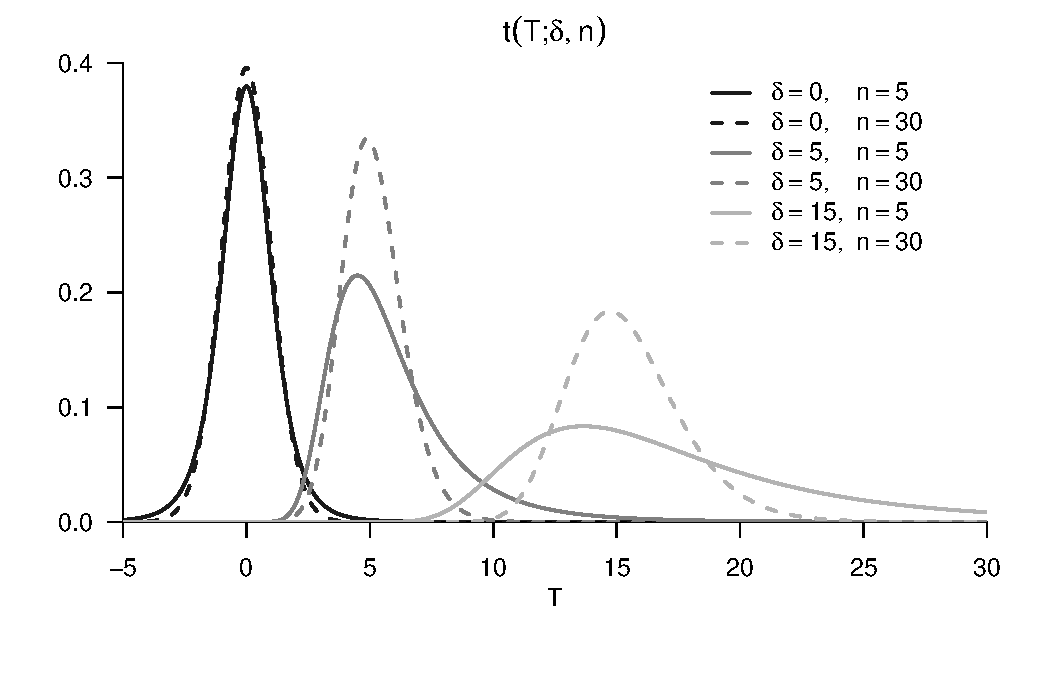
\includegraphics[width=0.8\linewidth]{12_Abbildungen/wtfi_12_nichtzentrale_t_verteilung} \end{center}
\end{frame}

\begin{frame}{Einstichproben-T-Test \textbar{} (2) Definition und
Analyse der Teststatistik}
\protect\hypertarget{einstichproben-t-test-2-definition-und-analyse-der-teststatistik-3}{}
\footnotesize
\begin{theorem}[Nichtzentrale T-Transformation]
\normalfont
\justifying
$\ups \sim N(\mu,1)$ sei eine normalverteilte Zufallsvariable, $U \sim \chi^2(n)$
sei eine $\chi^2$ Zufallsvariable mit Freiheitsgradparameter $n$, und $\ups$ und
$U$ seien unabhängige Zufallsvariablen. Dann ist die Zufallsvariable
\begin{equation}
T := \frac{\ups}{\sqrt{U/n}}
\end{equation}
eine nichtzentrale $t$-Zufallsvariable mit Nichtzentralitätsparameter $\mu$ und
Freiheitsgradparameter $n$, also $T \sim t(\mu,n)$.
\end{theorem}
\vspace{-2mm}

Bemerkung

\begin{itemize}
\tightlist
\item
  Wir verzichten auf einen Beweis.
\end{itemize}

\begin{center}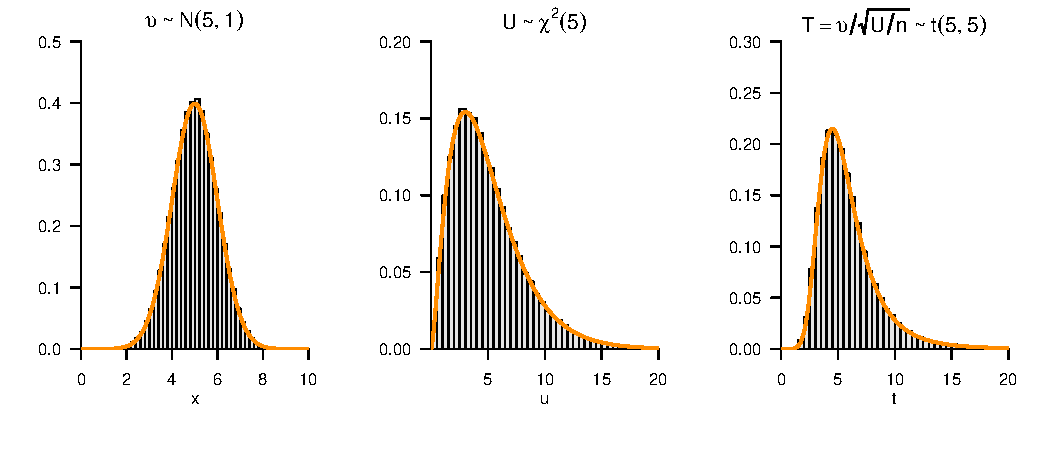
\includegraphics[width=0.8\linewidth]{12_Abbildungen/wtfi_12_nichtzentrale_t_transformation} \end{center}
\end{frame}

\begin{frame}{Einstichproben-T-Test \textbar{} (2) Definition und
Analyse der Teststatistik}
\protect\hypertarget{einstichproben-t-test-2-definition-und-analyse-der-teststatistik-4}{}
\footnotesize
\begin{theorem}[Verteilung der T-Teststatistik]
\justifying
\normalfont
$\ups_1,...,\ups_n \sim N(\mu,\sigma^2)$ sei die Stichprobe eines Normalverteilungmodells,
$\bar{\ups}$ sei das Stichprobenmittel, $S$ sei die Stichprobenstandardabweichung,
und es sei $\mu_0 \in \mathbb{R}$. Dann ist die  T-Teststatistik
\begin{equation}
T := \sqrt{n}\left(\frac{\bar{\ups} - \mu_0}{S} \right)
\end{equation}
eine nichtzentrale $t$-Zufallsvariable mit Nichtzentralitätsparameter
\begin{equation}
d = \sqrt{n}\left(\frac{\mu - \mu_0}{\sigma} \right)
\end{equation}
und Freiheitsgradparameter $n-1$, es gilt also $T \sim t(d,n-1)$
\end{theorem}

Bemerkung

\begin{itemize}
\tightlist
\item
  Wir verzichten auf einen Beweis.
\end{itemize}
\end{frame}

\begin{frame}{Einstichproben-T-Test \textbar{} (2) Definition und
Analyse der Teststatistik}
\protect\hypertarget{einstichproben-t-test-2-definition-und-analyse-der-teststatistik-5}{}
T-Teststatistik bei \(n = 12, \mu = 3, \sigma^2 = 2, \mu_0 = 0\)
\vspace{8mm}

\begin{center}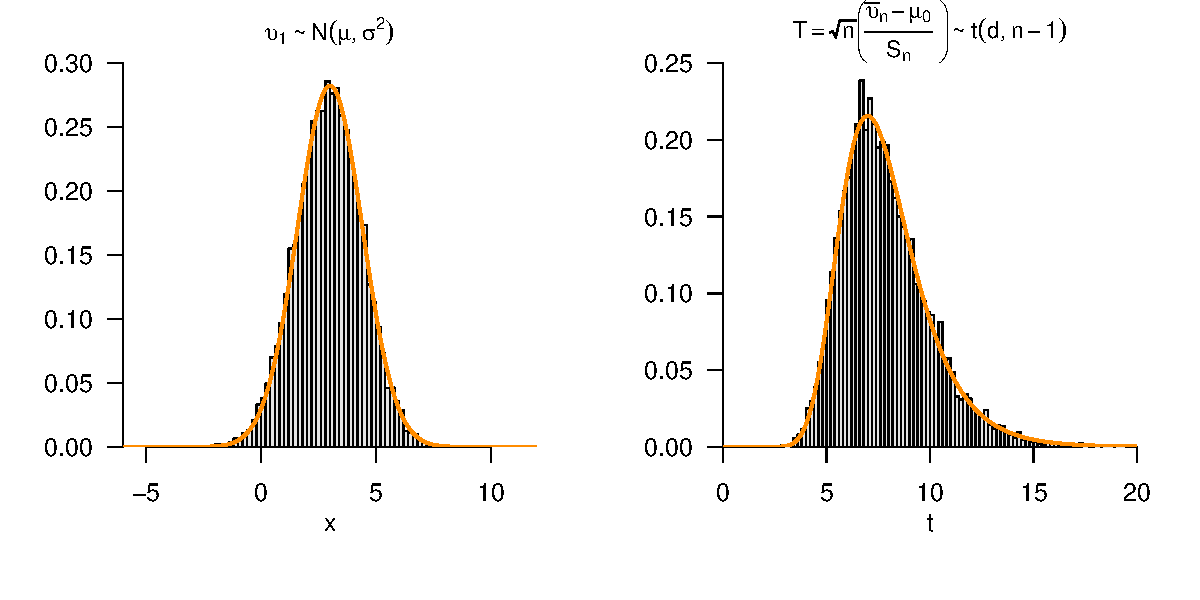
\includegraphics[width=1\linewidth]{12_Abbildungen/wtfi_12_t_teststatistik} \end{center}
\end{frame}

\begin{frame}{Einstichproben-T-Test \textbar{} (3) Definition des Tests}
\protect\hypertarget{einstichproben-t-test-3-definition-des-tests}{}
\vspace{5mm}

Vor dem Hintergrund des statistischen Modells des Einstichproben-T-Tests
betrachten wir die einfache Nullhypothese und die zusammengesetzte
Alternativhypothese \begin{equation}
H_0 : \mu = \mu_0 \Leftrightarrow \Theta_0 := \{\mu_0\}
\mbox{ und }
H_1 : \mu \neq \mu_0 \Leftrightarrow \Theta_1 := \mathbb{R} \setminus \{\mu_0\},
\end{equation} respektive, sowie die oben definierte T-Teststatistik
\begin{equation}
T := \sqrt{n}\left(\frac{\bar{\ups} - \mu_0}{S}\right).
\end{equation} \textbf{Wir definieren nun den zweiseitigen
Einstichproben-T-Test} \begin{equation}
\phi(\ups) := 1_{\{|T| \ge k\}} =
{\begin{cases}
1 & |T| \ge k \\
0 & |T|  <  k
\end{cases}}.
\end{equation}
\end{frame}

\begin{frame}{Einstichproben-T-Test \textbar{} (4) Analyse der
Testgütefunktion}
\protect\hypertarget{einstichproben-t-test-4-analyse-der-testguxfctefunktion}{}
\vspace{1cm}

\small
\begin{theorem}[Testgütefunktion]
\justifying
\normalfont
$\phi$ sei der im obend definierte Test. Dann ist die Testgütefunktion von $\phi$ gegeben durch
\begin{equation}
q_{\phi} : \mathbb{R} \to [0,1],
\mu \mapsto q_{\phi}(\mu)
:= 1 - \Psi(k;d_\mu,n-1) + \Psi(-k;d_\mu,n-1)
\end{equation}
wobei $\Psi(\cdot; d_\mu, n-1)$  die KVF der nichtzentralen $t$-Verteilung mit
Nichtzentralitätsparameter
\begin{equation}
d_\mu := \sqrt{n}\left(\frac{\mu - \mu_0}{\sigma}\right)
\end{equation}
und Freiheitsgradparameter $n-1$ bezeichnet.
\end{theorem}

Bemerkungen

\begin{itemize}
\tightlist
\item
  Wir visualisieren die Testgütefunktion unten in Abhängigkeit von
  \(k\).
\end{itemize}
\end{frame}

\begin{frame}{Einstichproben-T-Test \textbar{} (4) Analyse der
Testgütefunktion}
\protect\hypertarget{einstichproben-t-test-4-analyse-der-testguxfctefunktion-1}{}
\center Testgütefunktion \(q_\phi\) für
\(\sigma^2 = 9, \mu_0 = 4, n = 12\) und \(k = 1,2,3\). \vspace{2mm}
\begin{equation*}
\quad q_{\phi}(\mu) = \mathbb{P}_\mu(\phi = 1)
\end{equation*}

\begin{center}\includegraphics[width=0.8\linewidth]{12_Abbildungen/wtfi_12_t_test_ungerichtet_gütefunktion} \end{center}
\end{frame}

\begin{frame}{Einstichproben-T-Test \textbar{} (4) Analyse der
Testgütefunktion}
\protect\hypertarget{einstichproben-t-test-4-analyse-der-testguxfctefunktion-2}{}
\setstretch{1.2}

\footnotesize

\underline{Beweis}

Die Testgütefunktion des betrachteten Test im vorliegenden Testszenario
ist definiert als \begin{equation}
q_{\phi} : \mathbb{R} \to [0,1],
\mu \mapsto q_{\phi}(\mu) := \mathbb{P}_{\mu}(\phi = 1).
\end{equation} Da die Wahrscheinlichkeiten für \(\phi = 1\) und dafür,
dass die zugehörige Teststatistik im Ablehnungsbereich des Tests liegt
gleich sind, benötigen wird die also zunächst die Verteilung der
Teststatistik. Wir haben oben bereits gesehen, dass die T-Teststatistik
\begin{equation}
T := \sqrt{n}\left(\frac{\bar{\ups} - \mu_0}{S} \right)
\end{equation} unter der Annahme
\(\ups_1,...,\ups_n \sim N(\mu,\sigma^2)\) nach einer nichtzentralen
\(t\)-Verteilung \(t(d,n-1)\) mit Nichtzentralitätsparameter
\begin{equation}
d_\mu := \sqrt{n}\left(\frac{\mu - \mu_0}{\sigma}\right)
\end{equation} verteilt ist. Der Ablehnungsbereich des zweiseitigen
T-Tests ergibt sich zu \begin{equation}
A  = \,]-\infty, -k]\, \cup \,]k,\infty[.
\end{equation} \vfill
\end{frame}

\begin{frame}{Einstichproben-T-Test \textbar{} (4) Analyse der
Testgütefunktion}
\protect\hypertarget{einstichproben-t-test-4-analyse-der-testguxfctefunktion-3}{}
\setstretch{1.2}

\footnotesize

\underline{Beweis (fortgeführt)}

Mit diesem Ablehungsbereich ergibt sich dann \begin{align}
\begin{split}
q_\phi(\mu)
& = \mathbb{P}_{\mu}(\phi = 1)                                                   \\
& = \mathbb{P}_{\mu}\left(T \in ]-\infty, -k]\,
                         \cup \,]k,\infty[ \right)                               \\
& = \mathbb{P}_{\mu}\left(T \in ]-\infty, -k]\right)
  + \mathbb{P}_{\mu}\left(T \in [k,\infty[ \right)                               \\
& = \mathbb{P}_{\mu}(T \le -k)  + \mathbb{P}_{\mu}(T \ge k)                      \\
& = \mathbb{P}_{\mu}(T \le -k)  + (1-\mathbb{P}_{\mu}(T \le k))                  \\
& = 1 - \mathbb{P}_{\mu}(T \le k)  + \mathbb{P}_{\mu}(T \le - k)                 \\
& = 1 - \Psi(k; d_\mu, n-1)  + \Psi(-k;d_\mu,n-1),
\end{split}
\end{align} wobei \(\Psi(\cdot; d_\mu,n-1)\) die KVF der nichtzentralen
T-Verteilung mit Nichtzentralitätsparameter \(d_\mu\) und
Freiheitsgradparameter \(n-1\) bezeichnet.

\(\hfill\Box\) \vfill
\end{frame}

\begin{frame}{Einstichproben-T-Test \textbar{} (5) Testumfangkontrolle}
\protect\hypertarget{einstichproben-t-test-5-testumfangkontrolle}{}
\small
\begin{theorem}[Testumfangkontrolle]
\justifying
\normalfont
$\phi$ sei der oben definierte Test. Dann ist $\phi$ ein
Level-$\alpha_0$-Test mit Testumfang $\alpha_0$, wenn der kritische Wert
definiert ist durch
\begin{equation}
k_{\alpha_0} := \Psi^{-1}\left(1 - \frac{\alpha_0}{2}; n-1 \right),
\end{equation}
wobei $\Psi^{-1}(\cdot; n-1)$ die inverse KVF der $t$-Verteilung mit $n-1$
Freiheitsgraden ist.
\end{theorem}

\footnotesize

\underline{Beweis}

Damit der betrachtete Test ein Level-\(\alpha_0\)-Test ist, muss
bekanntlich \(q_\phi(\mu) \le \alpha_0\) für alle \(\mu \in \{\mu_0\}\),
also hier \(q_\phi(\mu_0) \le \alpha_0\), gelten. Weiterhin ist der
Testumfang des betrachteten Tests durch
\(\alpha = \max_{\mu \in \{\mu_0\}} q_\phi(\mu)\), also hier durch
\(\alpha = q_\phi(\mu_0)\) gegeben. Wir müssen also zeigen, dass die
Wahl von \(k_{\alpha_0}\) garantiert, dass \(\phi\) ein
Level-\(\alpha_0\)-Test mit Testumfang \(\alpha_0\) ist. Dazu merken wir
zunächst an, dass für \(\mu = \mu_0\) gilt, dass \begin{align}
\begin{split}
q_\phi(\mu_0)
& =  1 - \Psi(k;d_{\mu_0},n-1) + \Psi(-k;d_{\mu_0},n-1)                          \\
& =  1 - \Psi(k;0,n-1) + \Psi(-k;0,n-1)                                          \\
& =  1 - \Psi(k;n-1) + \Psi(-k;n-1),                                             \\
\end{split}
\end{align} wobei \(\Psi(\cdot;d,n-1)\) und \(\Psi(\cdot;n-1)\) die KVF
der nichtzentralen \(t\)-Verteilung mit Nichtzentralitätsparameter \(d\)
und Freiheitsgradparameter \(n-1\) sowie der \(t\)-Verteilung mit
Freiheitsgradparameter \(n-1\), respektive, bezeichnen.
\end{frame}

\begin{frame}{Einstichproben-T-Test \textbar{} (5) Testumfangkontrolle}
\protect\hypertarget{einstichproben-t-test-5-testumfangkontrolle-1}{}
\footnotesize

\underline{Beweis (fortgeführt)}

Sei nun also \(k := k_{\alpha_0}\). Dann gilt \begin{align}
\begin{split}
q_\phi(\mu_0)
& = 1 - \Psi(k_{\alpha_0};n-1) + \Psi(-k_{\alpha_0};n-1)                             \\
& = 1 - \Psi(k_{\alpha_0};n-1) + (1 - \Psi(k_{\alpha_0};n-1)                         \\
& = 2(1-\Psi(k_{\alpha_0};n-1))                                                      \\
& = 2\left(1-\Psi\left(\Psi^{-1}\left(1- \frac{\alpha_0}{2} , n-1\right), n-1\right)\right) \\
& = 2\left(1 - 1 + \alpha_0/2\right)                          \\
& = \alpha_0,
\end{split}
\end{align} wobei die zweite Gleichung mit der Symmetrie der
\(t\)-Verteilung folgt. Es folgt also direkt, dass bei der Wahl von
\(k = k_{\alpha_0}\), \(q_\phi(\mu_0)\le \alpha_0\) ist und der
betrachtete Test somit ein Level-\(\alpha_0\)-Test ist. Weiterhin folgt
direkt, dass der Testumfang des betrachteten Tests bei der Wahl von
\(k = k_{\alpha_0}\) gleich \(\alpha_0\) ist.
\end{frame}

\begin{frame}{Einstichproben-T-Test \textbar{} (5) Testumfangkontrolle}
\protect\hypertarget{einstichproben-t-test-5-testumfangkontrolle-2}{}
\small

\center Wahl von
\(k_{\alpha_0} := \Psi^{-1}(1- \frac{\alpha_0}{2}; n-1)\) mit \(n =12\),
\(\alpha_0 := 0.05\) und Ablehnungsbereich \vspace{3mm}

\begin{center}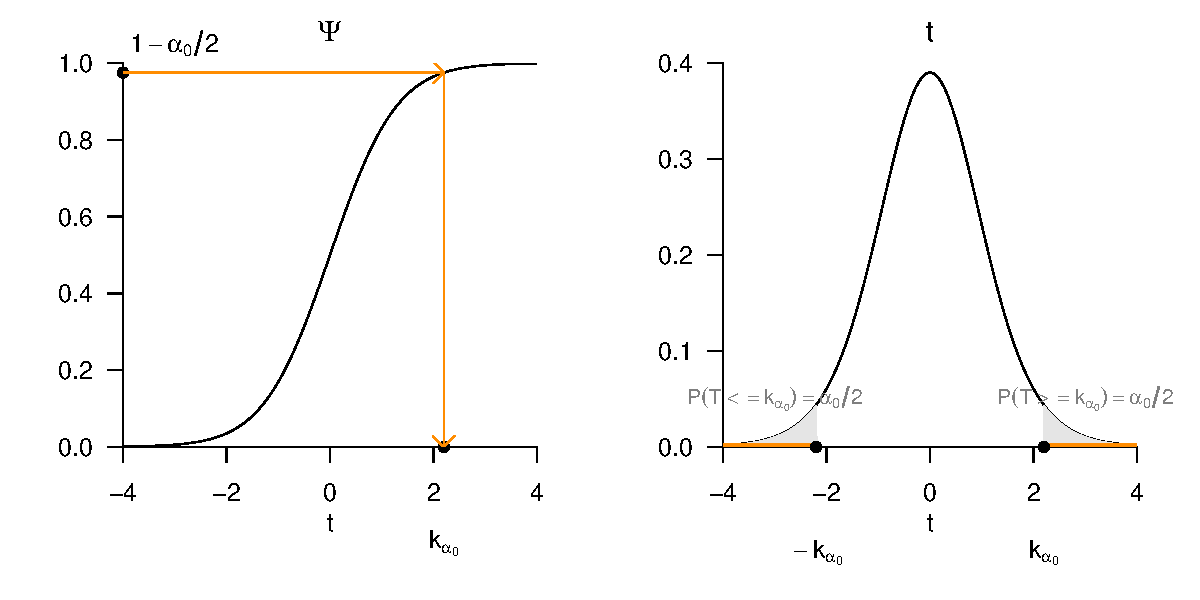
\includegraphics[width=1\linewidth]{12_Abbildungen/wtfi_12_t_test_ungerichtet_testumfangkontrolle} \end{center}
\end{frame}

\begin{frame}{Einstichproben-T-Test \textbar{} (5) Testumfangkontrolle}
\protect\hypertarget{einstichproben-t-test-5-testumfangkontrolle-3}{}
\justifying

\noindent \vspace{1mm} Praktisches Vorgehen \small

\begin{itemize}
\item
  \justifying Man nimmt an, dass ein vorliegender Datensatz
  \(y_1,...,y_n\) eine Realisation von
  \(\ups_1,...,\ups_n \sim N(\mu,\sigma^2)\) mit unbekannten Parametern
  \(\mu\) und \(\sigma^2 > 0\) ist.
\item
  Man möchte entscheiden ob für ein \(\mu_0 \in \mathbb{R}\) eher
  \(H_0 : \mu = \mu_0\) oder \(H_1: \mu \neq \mu_0\) zutrifft.

  \item

  Man wählt ein Signifikanzlevel \(\alpha_0\) und bestimmt den
  zugehörigen Freiheitsgradparameter-abhängigen kritischen Wert
  \(k_{\alpha_0}\). Zum Beispiel gilt bei Wahl von \(\alpha_0 := 0.05\)
  und \(n=12\), also Freiheitsgradparameter 11, dass
  \(k_{0.05}=\Psi^{-1}(1 - 0.05/2; 11) \approx 2.20\) ist.
\item
  Anhand von \(n, \mu_0, \bar{\ups}\) und \(s_n\) berechnet man die
  Realisierung der T-Teststatistik \begin{equation}
  t := \sqrt{n}\left(\frac{\bar{y} - \mu_0}{s}\right)
  \end{equation}
\item
  Wenn \(t\) größer-gleich \(k_{\alpha_0}\) ist oder wenn \(t\) kleiner-
  gleich \(-k_{\alpha_0}\) ist, lehnt man die Nullhypothese ab,
  andernfalls lehnt man sie nicht ab. Die oben entwickelte Theorie
  garantiert dann, dass man in höchstens \(\alpha_0 \cdot 100\) von
  \(100\) Fällen die Nullhypothese fälschlicherweise ablehnt.
\end{itemize}
\end{frame}

\begin{frame}[fragile]{Einstichproben-T-Test \textbar{} (5)
Testumfangkontrolle}
\protect\hypertarget{einstichproben-t-test-5-testumfangkontrolle-4}{}
Simulation des praktischen Vorgehens \vspace{2mm}

\tiny
\setstretch{1}

\begin{Shaded}
\begin{Highlighting}[]
\CommentTok{\# Modellparameter}
\NormalTok{n         }\OtherTok{=} \DecValTok{12}                                           \CommentTok{\# Anzahl der Datenpunkte}
\NormalTok{mu        }\OtherTok{=} \DecValTok{0}                                            \CommentTok{\# wahrer, aber unbekannter, Erwartungswertparameter}
\NormalTok{sigsqr    }\OtherTok{=} \DecValTok{2}                                            \CommentTok{\# wahrer, aber unbekannter, Varianzmatrixparameter}

\CommentTok{\# Testparameter}
\NormalTok{mu\_0      }\OtherTok{=} \DecValTok{0}                                            \CommentTok{\# H\_0 Hypothesenparameter, hier \textbackslash{}mu = \textbackslash{}mu\_0}
\NormalTok{alpha\_0   }\OtherTok{=} \FloatTok{0.05}                                         \CommentTok{\# Signifikanzlevel}
\NormalTok{k\_alpha\_0 }\OtherTok{=} \FunctionTok{qt}\NormalTok{(}\DecValTok{1}\SpecialCharTok{{-}}\NormalTok{alpha\_0}\SpecialCharTok{/}\DecValTok{2}\NormalTok{,n}\DecValTok{{-}1}\NormalTok{)                          }\CommentTok{\# kritischer Wert}

\CommentTok{\# Simulation der Testumfangkontrolle}
\FunctionTok{set.seed}\NormalTok{(}\DecValTok{1}\NormalTok{)                                              }\CommentTok{\# Random number generator seed}
\NormalTok{nsim      }\OtherTok{=} \FloatTok{1e6}                                          \CommentTok{\# Anzahl Simulationen}
\NormalTok{phi       }\OtherTok{=} \FunctionTok{rep}\NormalTok{(}\ConstantTok{NaN}\NormalTok{,nsim)                                }\CommentTok{\# Testentscheidungsarray}
\ControlFlowTok{for}\NormalTok{(j }\ControlFlowTok{in} \DecValTok{1}\SpecialCharTok{:}\NormalTok{nsim)\{                                        }\CommentTok{\# Simulationsiterationen}
\NormalTok{    y      }\OtherTok{=} \FunctionTok{rnorm}\NormalTok{(n,mu,sigsqr)                          }\CommentTok{\# \textbackslash{}ups\_i \textbackslash{}sim N(\textbackslash{}mu,\textbackslash{}Sigma), i = 1,...,n}
\NormalTok{    y\_bar  }\OtherTok{=} \FunctionTok{mean}\NormalTok{(y)                                     }\CommentTok{\# Stichprobenmittel}
\NormalTok{    s      }\OtherTok{=} \FunctionTok{sd}\NormalTok{(y)                                       }\CommentTok{\# Stichprobenstandardabweichung}
\NormalTok{    Tee    }\OtherTok{=} \FunctionTok{sqrt}\NormalTok{(n)}\SpecialCharTok{*}\NormalTok{((y\_bar }\SpecialCharTok{{-}}\NormalTok{ mu\_0)}\SpecialCharTok{/}\NormalTok{s)                  }\CommentTok{\# T{-}Teststatistik}
    \ControlFlowTok{if}\NormalTok{(}\FunctionTok{abs}\NormalTok{(Tee) }\SpecialCharTok{\textgreater{}}\NormalTok{ k\_alpha\_0)\{                            }\CommentTok{\# Test 1\_\{|t| \textgreater{}= k\_alpha\_0\}}
\NormalTok{        phi[j] }\OtherTok{=} \DecValTok{1}                                       \CommentTok{\# Ablehnen von H\_0}
\NormalTok{    \} }\ControlFlowTok{else}\NormalTok{ \{}
\NormalTok{        phi[j] }\OtherTok{=} \DecValTok{0}                                       \CommentTok{\# Nicht Ablehnen von H\_0}
\NormalTok{    \}}
\NormalTok{\}}

\CommentTok{\# Ausgabe}
\FunctionTok{cat}\NormalTok{(}\StringTok{"Kritischer Wert              ="}\NormalTok{, k\_alpha\_0,}
    \StringTok{"}\SpecialCharTok{\textbackslash{}n}\StringTok{Geschätzter Testumfang alpha ="}\NormalTok{, }\FunctionTok{mean}\NormalTok{(phi))}
\end{Highlighting}
\end{Shaded}

\begin{verbatim}
> Kritischer Wert              = 2.2 
> Geschätzter Testumfang alpha = 0.0498
\end{verbatim}
\end{frame}

\begin{frame}{Einstichproben-T-Test \textbar{} (6) Analyse der
Powerfunktion}
\protect\hypertarget{einstichproben-t-test-6-analyse-der-powerfunktion}{}
\vfill
\justifying

\small

Wir betrachten die Testgütefunktion \begin{equation}
q_\phi : \mathbb{R} \to [0,1],
\mu \mapsto q_\phi(\mu)
:= 1 - \Psi(k_{\alpha_0}; d_\mu, n-1) + \Psi(-k_{\alpha_0}; d_\mu, n-1)
\end{equation} bei kontrolliertem Testumfang, also für
\(k_{\alpha_0} := \Psi^{-1}(1-\alpha_0/2;n-1)\) mit festem \(\alpha_0\)
als Funktion des Nichtzentralitätsparameters und des Stichprobenumfangs.
Namentlich hängt hier \(k_{\alpha_0}\) auch von \(n\) ab.

Es ergibt sich die bivariate reellwertige Funktion \begin{equation}
\pi : \mathbb{R} \times \mathbb{N} \to [0,1],
(d,n) \mapsto
\pi(d,n) := 1 - \Psi(k_{\alpha_0}; d, n-1) + \Psi(-k_{\alpha_0}; d, n-1)
\end{equation} Bei festgelegten \(\alpha_0\) hängt die Powerfunktion des
zweiseitigen T-Tests mit einfacher Nullhypothese also vom unbekannten
Wert \(d\) und von der Stichprobengröße \(n\) ab. Wir visualisieren
diese Abhängigkeiten untenstehend. \vfill
\end{frame}

\begin{frame}{Einstichproben-T-Test \textbar{} (6) Analyse der
Powerfunktion}
\protect\hypertarget{einstichproben-t-test-6-analyse-der-powerfunktion-1}{}
\small

Powerfunktion für \(\alpha_0 = 0.05\)

\begin{center}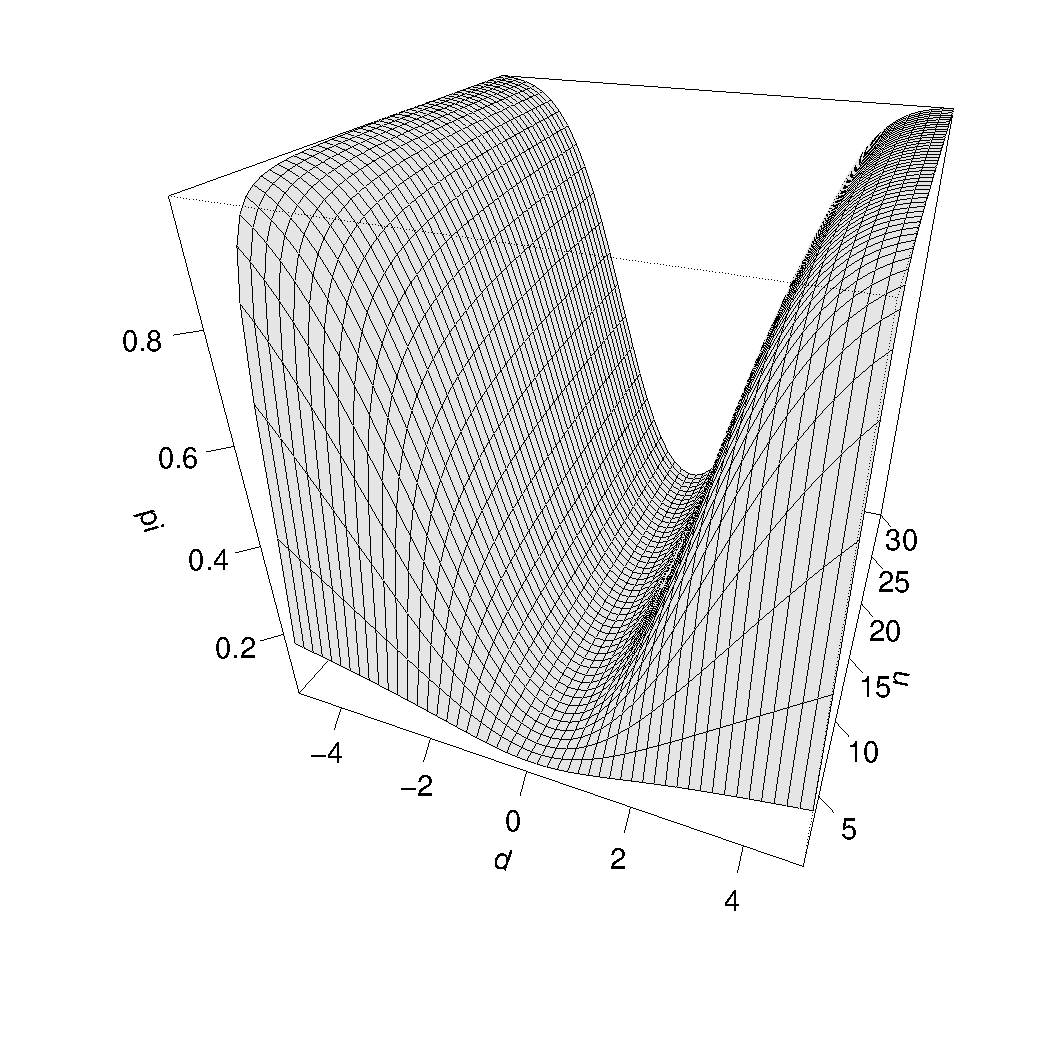
\includegraphics[width=0.6\linewidth]{12_Abbildungen/wtfi_12_t_test_ungerichtet_power_005} \end{center}
\end{frame}

\begin{frame}{Einstichproben-T-Test \textbar{} (6) Analyse der
Powerfunktion}
\protect\hypertarget{einstichproben-t-test-6-analyse-der-powerfunktion-2}{}
\small

Powerfunktion für \(\alpha_0 = 0.001\)

\begin{center}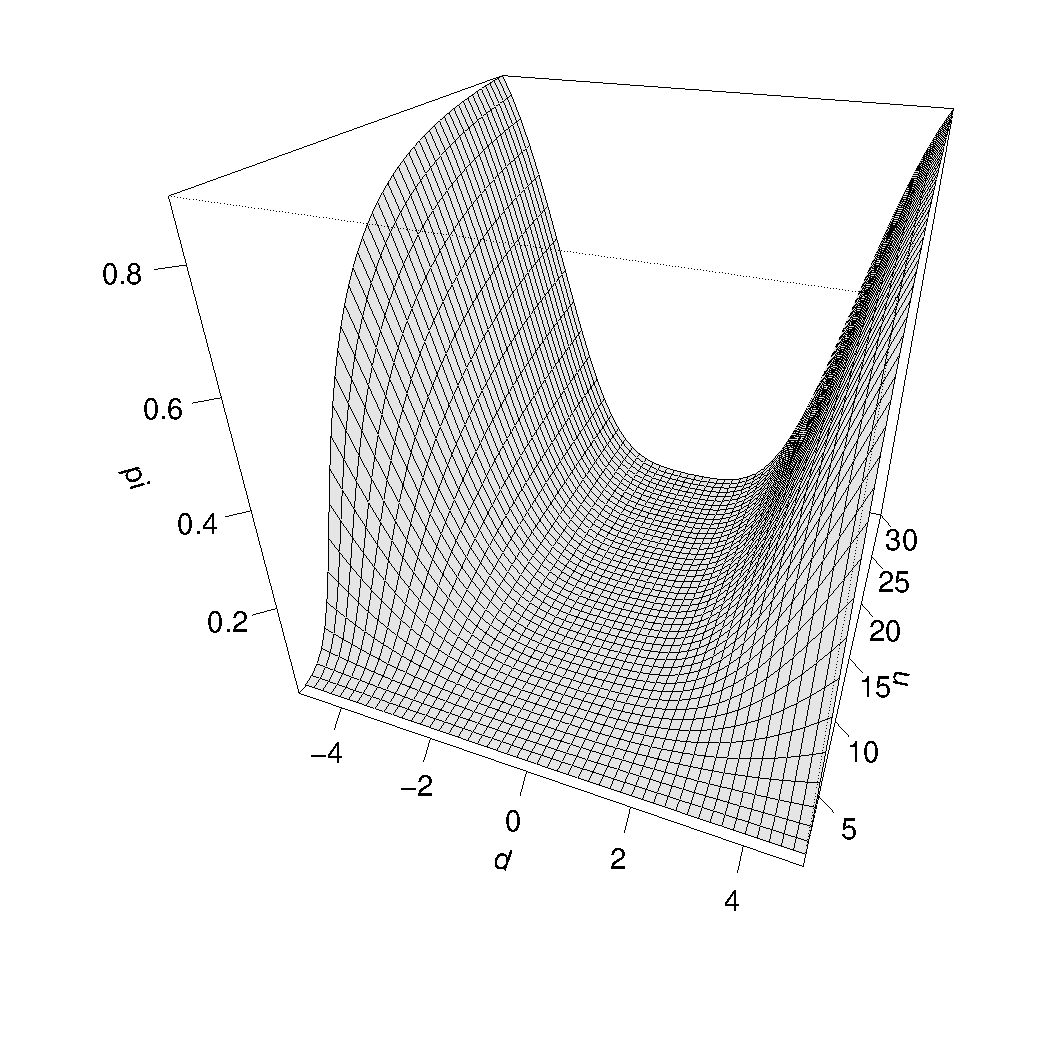
\includegraphics[width=0.6\linewidth]{12_Abbildungen/wtfi_12_t_test_ungerichtet_power_0001} \end{center}
\end{frame}

\begin{frame}{Einstichproben-T-Test \textbar{} (6) Analyse der
Powerfunktion}
\protect\hypertarget{einstichproben-t-test-6-analyse-der-powerfunktion-3}{}
\small
\justifying

Powerfunktionen für \(\mu_0 = 0\) \vspace{2mm}

\begin{center}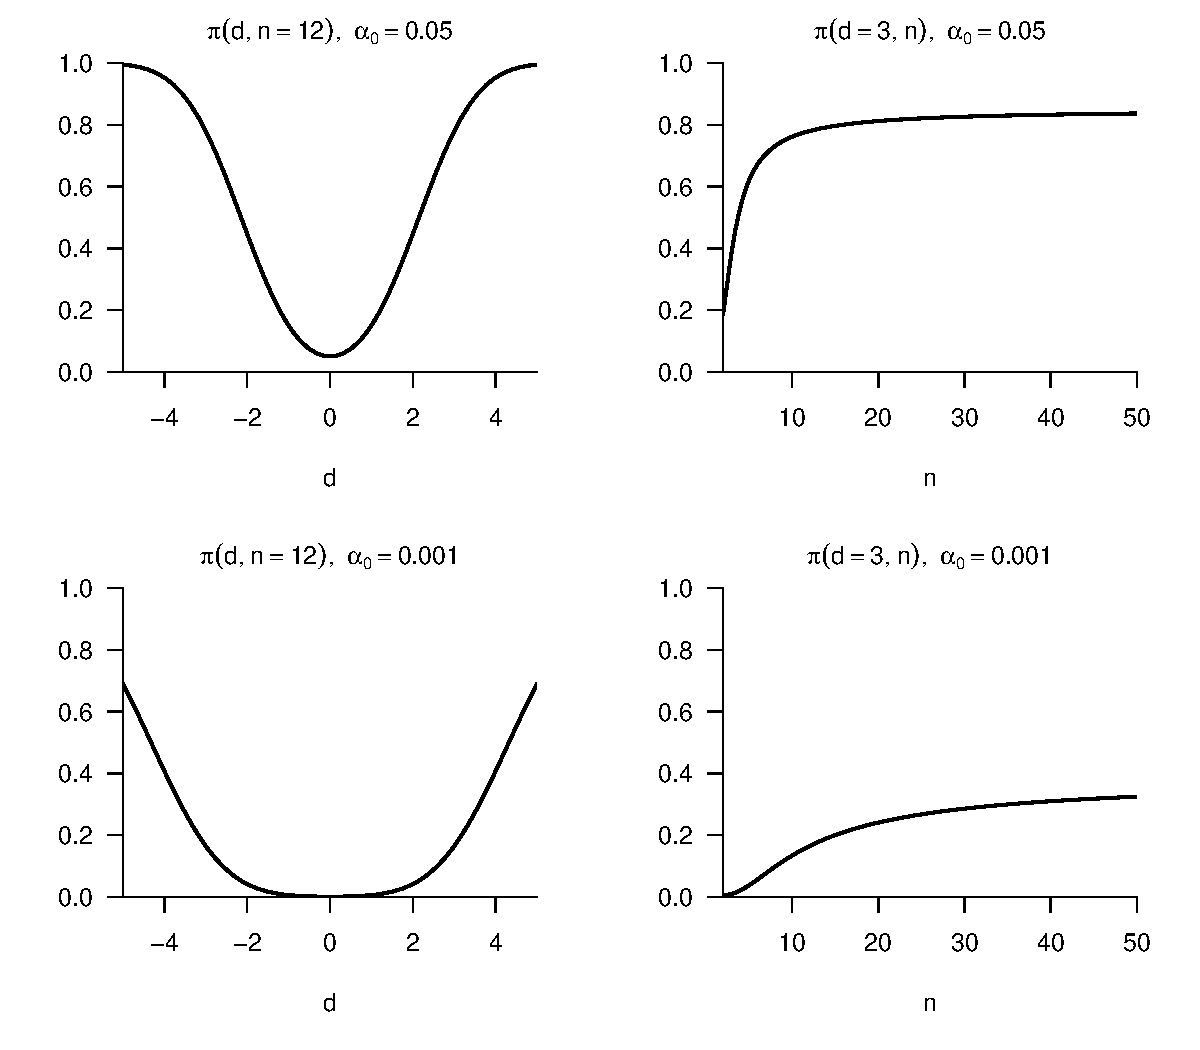
\includegraphics[width=0.7\linewidth]{12_Abbildungen/wtfi_12_t_test_ungerichtet_powerfunktionen} \end{center}
\end{frame}

\begin{frame}{Einstichproben-T-Test \textbar{} (6) Analyse der
Powerfunktion}
\protect\hypertarget{einstichproben-t-test-6-analyse-der-powerfunktion-4}{}
Praktisches Vorgehen \small

Mit größerem \(n\) steigt die Powerfunktion des Tests an

\begin{itemize}
\item
  Ein großer Stichprobenumfang ist besser als ein kleiner
  Stichprobenumfang.
\item
  Kosten für die Erhöhung des Stichprobenumfangs werden aber nicht
  berücksichtigt.
\end{itemize}

\(\Rightarrow\) Die Theorie statistischer Hypothesentests ist nicht
besonders lebensnah.

\vspace{1mm}

Die Powerfunktion hängt vom wahren, aber unbekannten, Parameterwert
\(d = \sqrt{n}(\mu - \mu_0)/\sigma\) ab.

\(\Rightarrow\) Wenn man \(d\) schon kennen würde, würde man den Test
nicht durchführen.

\vspace{1mm}

Generell wird folgendes Vorgehen favorisiert

\begin{itemize}
\item
  Man legt das Signifikanzlevel \(\alpha_0\) fest und evaluiert die
  Powerfunktion.
\item
  Man wählt einen Mindestparameterwert \(d^*\), den man mit
  \(\pi(d,n) = \beta\) detektieren möchte.
\item
  Ein konventioneller Wert ist \(\beta = 0.8\).
\item
  Man liest die für \(\pi(d = d^*,n) = \beta\) nötige Stichprobengröße
  \(n\) ab.
\end{itemize}
\end{frame}

\begin{frame}{Einstichproben-T-Test \textbar{} (6) Analyse der
Powerfunktion}
\protect\hypertarget{einstichproben-t-test-6-analyse-der-powerfunktion-5}{}
Praktisches Vorgehen \vspace{5mm}

\begin{center}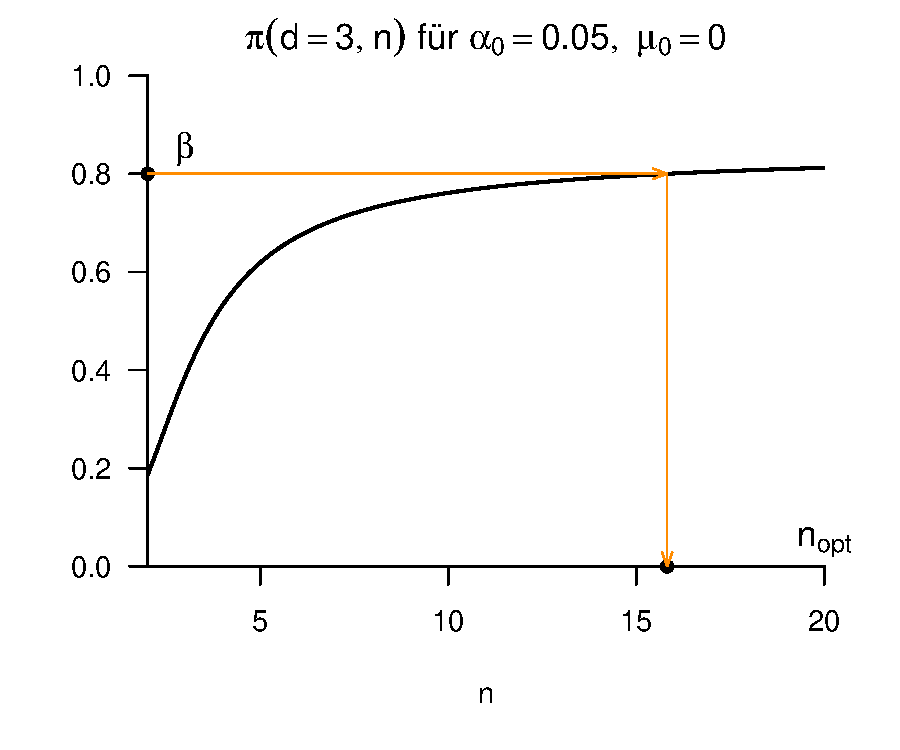
\includegraphics[width=0.6\linewidth]{12_Abbildungen/wtfi_12_t_test_ungerichtet_stichprobengröße} \end{center}
\end{frame}

\begin{frame}{}
\protect\hypertarget{section-9}{}
\setstretch{2.4}
\large
\vfill

Grundlegende Definitionen

Einstichproben-T-Test

\textbf{p-Werte}

Konfidenzintervalle und Hypothesentests

Anwendungsbeispiel

Selbstkontrollfragen \vfill
\end{frame}

\begin{frame}{p-Werte}
\protect\hypertarget{p-werte}{}
Motivation

\small
\begin{itemize}
\justifying
\item  Es werde ein zweiseitiger Einstichproben-T-Test mit $n = 12$ und $\alpha_0 = 0.05$ durchgeführt.
\begin{itemize}
\small
\item[$\circ$]  $H_0$ wird abgelehnt, wenn $|T| \ge 2.20$.
\end{itemize}
\item Nehmen wir an, es werde $t = 2.26$ beobachtet.
\begin{itemize}
\small
\item[$\circ$] Das Testergebnis lautet "$H_0$ Ablehnen".
\end{itemize}
\item Nehmen wir an, es werde $t = 3.81$ beobachtet.
\begin{itemize}
\small
\item[$\circ$] Das Testergebnis lautet "$H_0$ Ablehnen".
\end{itemize}
\item Der alleinige Bericht des Testergebnis supprimiert interessante Information.
\item[$\quad \Rightarrow$] Neben der Testumfangkontrolle durch z.B. $\alpha_0 = 0.05$
ist es daher üblich, alle Werte von $\alpha_0$ anzugeben, für die ein
Level-$\alpha_0$-Test zum Ablehnen von $H_0$ führen würde.
\begin{itemize}
\justifying
\small
\item[$\circ$] Bei $t = 2.26$ würde $H_0$ für jedes $\alpha_0$ mit $2.26 \ge \Psi^{-1}\left(1-\frac{\alpha_0}{2};11\right)$ abgelehnt werden.
\item[$\circ$] Bei $t = 3.81$ würde $H_0$ für jedes $\alpha_0$ mit $3.81 \ge \Psi^{-1}\left(1-\frac{\alpha_0}{2};11\right)$ abgelehnt werden.
\end{itemize}
\item Das kleinste Signifikanzlevel $\alpha_0$, bei dem man $H_0$ basierend auf
einem Wert der Teststatistik ablehnen würde, wird \textit{p-Wert} des Wertes 
der Teststatistik genannt.
\end{itemize}
\end{frame}

\begin{frame}{p-Werte}
\protect\hypertarget{p-werte-1}{}
\small
\begin{definition}[p-Wert]
\justifying
$\phi$ sei ein kritischer Wert-basierter Test. Der \textit{p-Wert} ist das
kleinste Signifikanzlevel $\alpha_0$, bei welchem man die Nullhypothese
basierend auf einem vorliegendem Wert der Teststatistik ablehnen würde.
\end{definition}
\small

Beispiel (Zweiseitiger Einstichproben-T-Test mit einfacher
Nullhypothese)

\footnotesize

\begin{itemize}
\tightlist
\item
  Bei \(T = t\) würde \(H_0\) für jedes \(\alpha_0\) mit
  \(|t| \ge \Psi^{-1}\left(1- \frac{\alpha_0}{2};n-1\right)\) abgelehnt
  werden. Für diese \(\alpha_0\) gilt, wie unten gezeigt,
  \begin{equation}
  \alpha_0 \ge 2 \mathbb{P}(T \ge |t|).
  \end{equation}
\item
  Das kleinste \(\alpha_0 \in [0,1]\) mit
  \(\alpha_0 \ge 2 \mathbb{P}(T \ge |t|)\) ist dann
  \(\alpha_0 = 2 \mathbb{P}(T \ge |t|)\), also folgt \begin{equation}
  \mbox{p-Wert} =  2 \mathbb{P}(T \ge |t|) = 2(1 - \Psi(|t|;n-1)).
  \end{equation}
\item
  Zum Beispiel ist bei \(n = 12\) für \(T = 2.26\) der p-Wert \(0.045\),
  für \(T = -2.26\) ist der p-Wert auch \(0.045\), für \(T = 3.81\) ist
  der p-Wert \(0.003\) und für \(T = -3.81\) ist der p-Wert auch
  \(0.003\).
\end{itemize}
\end{frame}

\begin{frame}{p-Werte}
\protect\hypertarget{p-werte-2}{}
\small

Beispiel (Zweiseitiger Einstichproben-T-Test mit einfacher
Nullhypothese)

\footnotesize

\begin{itemize}
\item
  \itemsep2mm \justifying Es bleibt zu zeigen, dass gilt
  \begin{equation}
  |t| \ge \Psi^{-1}(1- \frac{\alpha_0}{2}; n-1)
  \Leftrightarrow
  \alpha_0 \ge 2 \mathbb{P}(T \ge |t|)
  \end{equation}
\item
  Dies aber folgt aus \footnotesize \vspace{-2mm} \begin{align}
  \begin{split}
  |t|
  & \ge \Psi^{-1}\left(1 - \frac{\alpha_0}{2}; n-1\right)
  \\\Leftrightarrow
  \Psi(|t|; n-1)
  & \ge \Psi\left(\Psi^{-1}\left(1 - \frac{\alpha_0}{2}; n-1\right); n-1\right)
  \\\Leftrightarrow
  \Psi(|t|; n-1)
  & \ge 1 - \frac{\alpha_0}{2}
  \\\Leftrightarrow
  \mathbb{P}(T \le |t|)
  & \ge 1 - \frac{\alpha_0}{2}
  \\\Leftrightarrow
  \frac{\alpha_0}{2}
  & \ge 1 - \mathbb{P}(T \le |t|)
  \\\Leftrightarrow
  \frac{\alpha_0}{2}
  & \ge \mathbb{P}(T \ge |t|)
  \\\Leftrightarrow
  \alpha_0
  & \ge 2 \mathbb{P}(T \ge |t|).
  \end{split}
  \end{align}
\end{itemize}
\end{frame}

\begin{frame}{p-Werte}
\protect\hypertarget{p-werte-3}{}
\small

Beispiel (Zweiseitiger Einstichproben-T-Test mit einfacher
Nullhypothese) \vspace{8mm}

\vspace{3mm}

\begin{center}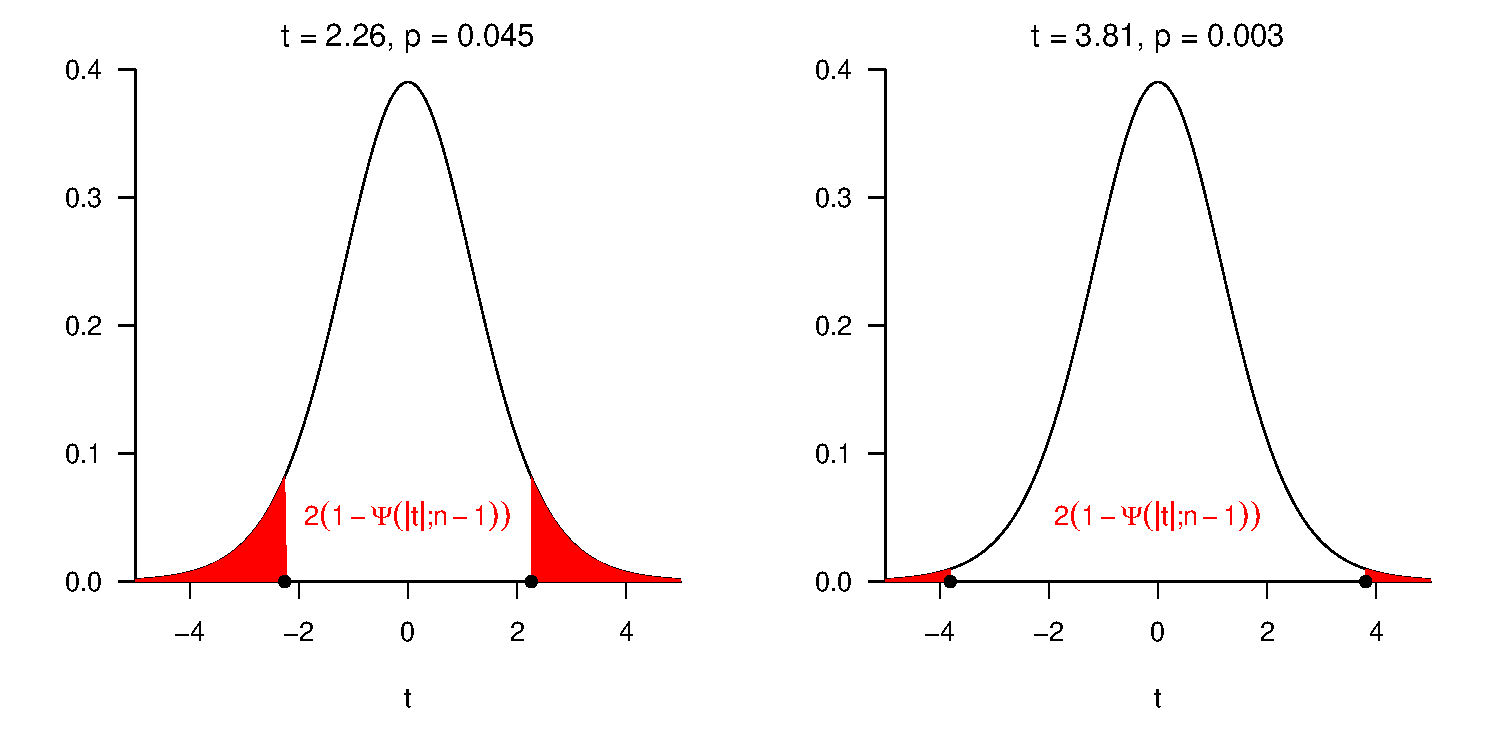
\includegraphics[width=1\linewidth]{12_Abbildungen/wtfi_12_p_werte} \end{center}
\end{frame}

\begin{frame}{p-Werte}
\protect\hypertarget{p-werte-4}{}
\small

Bemerkungen

\begin{itemize}
\justifying
\item[$\circ$] p-Werte spiegeln die Antwort auf die intuitive Frage wie
wahrscheinlich es im Frequentistischen Sinne wäre, den beobachteten oder einen
extremeren Wert der Teststatistik unter der Annahme eines Nullmodels zu
observieren.
\item[$\circ$] p-Werte sind ist extrem populär, ihre uninformierte Benutzung ist aber auch sehr umstritten.
\footnotesize
\item[$\rightarrow$] \href{https://www.tandfonline.com/toc/utas20/73/sup1}{The American Statistician (2019) Statistical Inference in the 21st Century: A World Beyond p < 0.05}
\small
\item[$\circ$]  p-Werte werden, wie Hypothesentestergebnisse generell, leider oft überinterpretiert.
\item[$\circ$]  Es gibt basierend auf dem Gesagten keinen Grund dies anzunehmen, trotzdem vorsorglich:
\begin{itemize}
\begin{footnotesize}
\item[$\circ$] p-Werte quantifizieren nicht die Wahrscheinlichkeit, dass die Nullhypothese wahr ist.
\item[$\circ$] Aufgrund von $p < 0.05$ sollte man nicht glauben, dass ein Effekt existiert.
\item[$\circ$] Aufgrund von $p > 0.05$ sollte man nicht glauben, dass ein Effekt nicht existiert.
\end{footnotesize}
\end{itemize}
\item[$\circ$] p-Werte sind eine Möglichkeit ein Signal-zu-Rauschen Verhältnis zu quantifizieren.
\item[$\circ$] p-Werte sind eine Möglichkeit Unsicherheit zu quantifizieren.
\end{itemize}
\end{frame}

\begin{frame}{}
\protect\hypertarget{section-10}{}
\setstretch{2.4}
\large
\vfill

Grundlegende Definitionen

Einstichproben-T-Test

p-Werte

\textbf{Konfidenzintervalle und Hypothesentests}

Anwendungsbeispiel

Selbstkontrollfragen \vfill
\end{frame}

\begin{frame}{Konfidenzintervalle und Hypothesentests}
\protect\hypertarget{konfidenzintervalle-und-hypothesentests}{}
\small
\begin{theorem}[Dualität von Konfidenzintervallen und Hypothesentest]
\justifying
\normalfont
$\ups = \ups_1,...,\ups_n \sim p_\theta$ sei eine Stichprobe mit Ergebnisraum
$\mathcal{Y}$ und Parameterraum $\Theta$. Weiterhin sei $[G_u(\ups), G_o(\ups)]$
ein $\delta$-Konfidenzintervall für $\theta$. Dann ist der Hypothesentest
\begin{equation}
\phi_\theta : \mathcal{Y} \to \{0,1\},
y \mapsto \phi(y)
:=
\begin{cases}
0, & [G_u(y), G_o(y)] \ni    \theta_0 \\
1, & [G_u(y), G_o(y)] \niton \theta_0 \\
\end{cases}
\end{equation}
ein Test vom Signifikanzlevel $\alpha_0 = 1 - \delta$ für die Hypothesen
\begin{equation}
\Theta_0 := \{\theta_0\} \mbox{ und } \Theta_1 := \Theta \setminus \{\theta_0\}.
\end{equation}
\end{theorem}

\footnotesize

\underline{Beweis} \vspace{1mm}

Aufgrund der einfachen Nullhypothese und somit \(\alpha_0 = \alpha\)
folgt \begin{equation}
\alpha_0
= \alpha
= \mathbb{P}_{\theta_0}(\phi(\ups) = 1)
= \mathbb{P}_{\theta_0}([G_u(y), G_o(y)] \niton \theta)
= 1 - \mathbb{P}_{\theta_0}([G_u(y), G_o(y)] \ni \theta)
= 1 - \delta.
\end{equation}

Bemerkung

\begin{itemize}
\tightlist
\item
  Mit \(\delta\)-Konfidenzintervallen kann man also Hypothesentests mit
  Signifikanzlevel \(\alpha_0 = 1-\delta\) konstruieren.
\end{itemize}
\end{frame}

\begin{frame}{Konfidenzintervalle und Hypothesentests}
\protect\hypertarget{konfidenzintervalle-und-hypothesentests-1}{}
\small

Beispiel (Konstruktion eines Hypothesentests aus einem
Konfidenzintervall)

\footnotesize

Wir haben bereits gesehen, dass für eine Stichprobe
\(\ups = \ups_1,...,\ups_n \sim N(\mu,\sigma^2)\), \(\delta \in ]0,1[\)
und \begin{equation}
t_\delta := \Psi^{-1}\left(\frac{1 + \delta}{2}; n-1 \right)
\end{equation} ein \(\delta\)-Konfidenzintervall durch \begin{equation}
\kappa :=
\left[\bar{\ups} - \frac{S}{\sqrt{n}}t_\delta,\bar{\ups} + \frac{S}{\sqrt{n}}t_\delta\right].
\end{equation} definiert ist. Mit der Dualität von Konfidenzintervallen
und Hypothesentests können wir also folgenden Test für die Hypothesen
\(\Theta_0 = \{\mu_0\}\) und \(\Theta_1 = \mathbb{R} \setminus \mu_0\)
definieren: \begin{equation}
\phi : \mathcal{Y} \to \{0,1\},
y \mapsto \phi(y)
:=
\begin{cases}
0, & \left[\bar{\ups} - \frac{S}{\sqrt{n}}t_\delta,\bar{\ups} + \frac{S}{\sqrt{n}}t_\delta\right]
           \ni \mu_0
          \\ \\
1, &\left[\bar{\ups} - \frac{S}{\sqrt{n}}t_\delta,\bar{\ups} + \frac{S}{\sqrt{n}}t_\delta\right]
          \niton \mu_0
          \\
\end{cases}
\end{equation} Dann gilt \begin{align}
\begin{split}
\mathbb{P}_{\mu_0}\left(\phi(\ups) = 1 \right)
& = 1 - \mathbb{P}_{\mu_0}\left(\phi(\ups) = 0 \right) \\
& = 1 - \mathbb{P}_{\mu_0}\left(
            \left[\bar{\ups} - \frac{S}{\sqrt{n}}t_\delta,
                  \bar{\ups} + \frac{S}{\sqrt{n}}t_\delta\right]
            \ni \mu_0\right) \\
& = 1 - \delta.
\end{split}
\end{align} und wir haben gezeigt, dass \(\phi\) ein Test vom
Signifikanzlevel \(\alpha_0 = 1 -\delta\) ist.
\end{frame}

\begin{frame}[fragile]{Konfidenzintervalle und Hypothesentests}
\protect\hypertarget{konfidenzintervalle-und-hypothesentests-2}{}
\vspace{2mm}

Simulation der Dualität von Konfidenzintervallen und Hypothesentests
\vspace{1mm} \tiny \setstretch{.9}

\begin{Shaded}
\begin{Highlighting}[]
\CommentTok{\# Modellformulierung}
\NormalTok{n       }\OtherTok{=} \DecValTok{12}                                          \CommentTok{\# Stichprobengröße}
\NormalTok{mu      }\OtherTok{=} \DecValTok{2}                                           \CommentTok{\# wahrer, aber unbekannter, Erwartungswertparameter}
\NormalTok{sigsqr  }\OtherTok{=} \DecValTok{1}                                           \CommentTok{\# wahrer, aber unbekannter, Varianzparameter}

\CommentTok{\# Konfidenzintervallparameter und Testparameter}
\NormalTok{delta   }\OtherTok{=} \FloatTok{0.95}                                        \CommentTok{\# Konfidenzbedingung}
\NormalTok{t\_delta }\OtherTok{=} \FunctionTok{qt}\NormalTok{((}\DecValTok{1}\SpecialCharTok{+}\NormalTok{delta)}\SpecialCharTok{/}\DecValTok{2}\NormalTok{, n}\DecValTok{{-}1}\NormalTok{)                        }\CommentTok{\# \textbackslash{}Psi\^{}\{{-}1\}((\textbackslash{}delta + 1)/2, n{-}1)}
\NormalTok{mu\_0    }\OtherTok{=}\NormalTok{ mu                                          }\CommentTok{\# Nullhypothesenparameter }

\CommentTok{\# Simulationen}
\FunctionTok{set.seed}\NormalTok{(}\DecValTok{1}\NormalTok{)                                           }\CommentTok{\# random number generator seed}
\NormalTok{ns      }\OtherTok{=} \FloatTok{1e2}                                         \CommentTok{\# Anzahl Simulationen}
\NormalTok{y\_bar   }\OtherTok{=} \FunctionTok{rep}\NormalTok{(}\ConstantTok{NaN}\NormalTok{,ns)                                 }\CommentTok{\# Stichprobenmittelarray}
\NormalTok{s       }\OtherTok{=} \FunctionTok{rep}\NormalTok{(}\ConstantTok{NaN}\NormalTok{,ns)                                 }\CommentTok{\# Stichprobenstandardabweichungarray}
\NormalTok{kappa   }\OtherTok{=} \FunctionTok{matrix}\NormalTok{(}\FunctionTok{rep}\NormalTok{(}\ConstantTok{NaN}\NormalTok{,}\DecValTok{2}\SpecialCharTok{*}\NormalTok{ns), }\AttributeTok{ncol =} \DecValTok{2}\NormalTok{)             }\CommentTok{\# Konfidenzintervallarray}
\NormalTok{kfn     }\OtherTok{=} \FunctionTok{rep}\NormalTok{(}\ConstantTok{NaN}\NormalTok{,ns)                                 }\CommentTok{\# Überdeckungsindikatorarray}
\NormalTok{phi     }\OtherTok{=} \FunctionTok{rep}\NormalTok{(}\ConstantTok{NaN}\NormalTok{,ns)                                 }\CommentTok{\# Testarray}
\ControlFlowTok{for}\NormalTok{(i }\ControlFlowTok{in} \DecValTok{1}\SpecialCharTok{:}\NormalTok{ns)\{                                       }\CommentTok{\# Simulationsiterationen}
  \CommentTok{\# Stichprobenrealisation und Konfidezintervallevaluation  }
\NormalTok{  y          }\OtherTok{=} \FunctionTok{rnorm}\NormalTok{(n,mu\_0,}\FunctionTok{sqrt}\NormalTok{(sigsqr))             }\CommentTok{\# Stichprobenrealisierung}
\NormalTok{  y\_bar[i]   }\OtherTok{=} \FunctionTok{mean}\NormalTok{(y)                                }\CommentTok{\# Stichprobenmittel}
\NormalTok{  s[i]       }\OtherTok{=} \FunctionTok{sd}\NormalTok{(y)                                  }\CommentTok{\# Stichprobenstandardabweichung}
\NormalTok{  kappa[i,}\DecValTok{1}\NormalTok{] }\OtherTok{=}\NormalTok{ y\_bar[i] }\SpecialCharTok{{-}}\NormalTok{ (s[i]}\SpecialCharTok{/}\FunctionTok{sqrt}\NormalTok{(n))}\SpecialCharTok{*}\NormalTok{t\_delta      }\CommentTok{\# untere KI Grenze}
\NormalTok{  kappa[i,}\DecValTok{2}\NormalTok{] }\OtherTok{=}\NormalTok{ y\_bar[i] }\SpecialCharTok{+}\NormalTok{ (s[i]}\SpecialCharTok{/}\FunctionTok{sqrt}\NormalTok{(n))}\SpecialCharTok{*}\NormalTok{t\_delta      }\CommentTok{\# obere KI Grenze}

  \CommentTok{\# Überdeckungs{-} und Testevaluation}
  \ControlFlowTok{if}\NormalTok{(kappa[i,}\DecValTok{1}\NormalTok{] }\SpecialCharTok{\textless{}=}\NormalTok{ mu\_0 }\SpecialCharTok{\&}\NormalTok{ mu\_0 }\SpecialCharTok{\textless{}=}\NormalTok{ kappa[i,}\DecValTok{2}\NormalTok{])\{}
\NormalTok{      kfn[i] }\OtherTok{=} \DecValTok{1}\NormalTok{\} }\ControlFlowTok{else}\NormalTok{\{kfn[i] }\OtherTok{=} \DecValTok{0}\NormalTok{\}                    }\CommentTok{\# Überdeckungsindikatorevaluation}
  \ControlFlowTok{if}\NormalTok{(kappa[i,}\DecValTok{1}\NormalTok{] }\SpecialCharTok{\textless{}=}\NormalTok{ mu\_0 }\SpecialCharTok{\&}\NormalTok{ mu\_0 }\SpecialCharTok{\textless{}=}\NormalTok{ kappa[i,}\DecValTok{2}\NormalTok{])\{}
\NormalTok{      phi[i] }\OtherTok{=} \DecValTok{0}\NormalTok{\} }\ControlFlowTok{else}\NormalTok{\{phi[i] }\OtherTok{=} \DecValTok{1}\NormalTok{\}\}                    }\CommentTok{\# Testevaluation}

\CommentTok{\# Ausgabe}
\FunctionTok{cat}\NormalTok{(   }\StringTok{"Geschätztes Konfidenzniveau ="}\NormalTok{, }\FunctionTok{mean}\NormalTok{(kfn),}
     \StringTok{"}\SpecialCharTok{\textbackslash{}n}\StringTok{Geschätzter Testumfang      ="}\NormalTok{, }\FunctionTok{mean}\NormalTok{(phi))}
\end{Highlighting}
\end{Shaded}

\begin{verbatim}
> Geschätztes Konfidenzniveau = 0.96 
> Geschätzter Testumfang      = 0.04
\end{verbatim}
\end{frame}

\begin{frame}{Konfidenzintervalle und Hypothesentests}
\protect\hypertarget{konfidenzintervalle-und-hypothesentests-3}{}
\vspace{1mm}

Simulation der Dualität von Konfidenzintervallen und Hypothesentests
\vspace{1mm}

\begin{center}\includegraphics[width=1\linewidth]{12_Abbildungen/wtfi_12_dualität} \end{center}
\end{frame}

\begin{frame}{}
\protect\hypertarget{section-11}{}
\setstretch{2.4}
\large
\vfill

Grundlegende Definitionen

Einstichproben-T-Test

p-Werte

Konfidenzintervalle und Hypothesentests

\textbf{Anwendungsbeispiel}

Selbstkontrollfragen \vfill
\end{frame}

\begin{frame}{Anwendungsbeispiel}
\protect\hypertarget{anwendungsbeispiel}{}
Beispiel \textbar{} Evidenzbasierte Evaluation von Psychotherapie bei
Depression

\begin{center}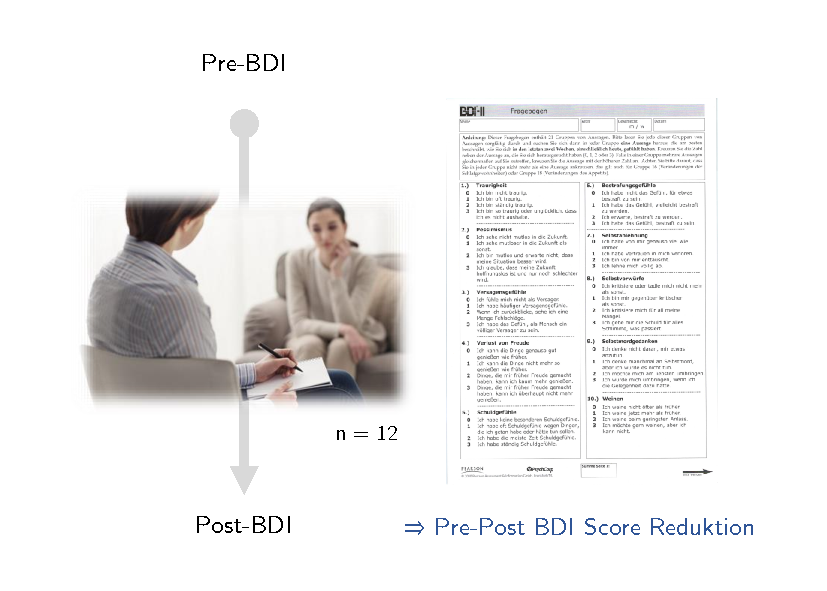
\includegraphics[width=0.8\linewidth]{12_Abbildungen/wtfi_12_messplan} \end{center}
\end{frame}

\begin{frame}{Einstichproben-T-Test}
\protect\hypertarget{einstichproben-t-test-5}{}
Beispiel \textbar{} Evidenzbasierte Evaluation von Psychotherapie bei
Depression \vspace{2mm}

\small

Wir legen für die BDI Score Reduktion \(\ups_i\) der \(i\)ten von \(n\)
Patient:innen das Modell \begin{equation}
\ups_{i} = \mu + \varepsilon_{i} \mbox{ mit } \varepsilon_{i} \sim N(0,\sigma^2) \mbox{ u.i.v. für } i = 1,...,n
\end{equation} zugrunde.

Wir erklären die BDI Reduktion \(\ups_i\) der \(i\)ten Patient:in also
mithilfe einer über die Gruppe von Patient:innen identischen BDI Score
Reduktion \(\mu\) als Effekt der Therapieintervention und einer
Patient:innen-spezifischen normalverteilten BDI Score
Reduktionsabweichung \(\varepsilon_{i}\), die sich aus sehr vielen
additiven Prozessen zusammensetzt, für die wir also eine
Normalverteilungsannahme treffen, und deren Varianz wir mit \(\sigma^2\)
parameterisieren.

Vor dem Hintergrund dieses Modells evaluieren wir die drei
Standardprobleme der Frequentistischen Inferenz für den Effekt der
Therapieintervention \(\mu\):

\begin{enumerate}
[(1)]
\tightlist
\item
  Was ist unserer Schätzung für den Effekt \(\mu\) der Therapie auf die
  BDI Score Reduktion?
\item
  Welches 95\%-Konfidenzintervall ist mit dieser Schätzung von \(\mu\)
  assoziiert?
\item
  Entscheiden wir uns sinnvoller Weise für die Nullhypothese
  \(\mu = 0\)?
\end{enumerate}
\end{frame}

\begin{frame}[fragile]{Anwendungsbeispiel}
\protect\hypertarget{anwendungsbeispiel-1}{}
Beispiel \textbar{} Evidenzbasierte Evaluation von Psychotherapie bei
Depression \vspace{2mm}

\footnotesize

\begin{Shaded}
\begin{Highlighting}[]
\NormalTok{fname }\OtherTok{=} \FunctionTok{file.path}\NormalTok{(}\FunctionTok{getwd}\NormalTok{(), }\StringTok{"12\_Hypothesentests.csv"}\NormalTok{)}
\NormalTok{D     }\OtherTok{=} \FunctionTok{read.table}\NormalTok{(fname, }\AttributeTok{sep =} \StringTok{","}\NormalTok{, }\AttributeTok{header =}\NormalTok{ T)}
\end{Highlighting}
\end{Shaded}

\vspace{2mm}

\begin{longtable}[]{@{}rr@{}}
\toprule()
i & BDI.Reduktion \\
\midrule()
\endhead
1 & -1 \\
2 & 3 \\
3 & -2 \\
4 & 9 \\
5 & 3 \\
6 & -2 \\
7 & 4 \\
8 & 5 \\
9 & 5 \\
10 & 1 \\
11 & 9 \\
12 & 4 \\
\bottomrule()
\end{longtable}
\end{frame}

\begin{frame}[fragile]{Anwendungsbeispiel}
\protect\hypertarget{anwendungsbeispiel-2}{}
Beispiel \textbar{} Evidenzbasierte Evaluation von Psychotherapie bei
Depression \vspace{2mm} \tiny \setstretch{1}

\begin{Shaded}
\begin{Highlighting}[]
\CommentTok{\# Einlesen und Auswahl der Daten}
\NormalTok{fname     }\OtherTok{=} \FunctionTok{file.path}\NormalTok{(}\FunctionTok{getwd}\NormalTok{(), }\StringTok{"12\_Hypothesentests.csv"}\NormalTok{)  }\CommentTok{\# Dateiname}
\NormalTok{D         }\OtherTok{=} \FunctionTok{read.table}\NormalTok{(fname, }\AttributeTok{sep =} \StringTok{","}\NormalTok{, }\AttributeTok{header =}\NormalTok{ T)      }\CommentTok{\# Dataframe}
\NormalTok{y         }\OtherTok{=}\NormalTok{ D}\SpecialCharTok{$}\NormalTok{BDI.Reduktion                               }\CommentTok{\# Datenrealisation}
\NormalTok{n         }\OtherTok{=} \FunctionTok{length}\NormalTok{(y)                                     }\CommentTok{\# Anzahl Datenpunkte}

\CommentTok{\# Parameterschätzung}
\NormalTok{y\_bar      }\OtherTok{=} \FunctionTok{mean}\NormalTok{(y)                                      }\CommentTok{\# Stichprobenmittel}
\NormalTok{mu\_hat     }\OtherTok{=}\NormalTok{ y\_bar                                        }\CommentTok{\# Unverzerrte Maximum{-}Likelihood Schätzung}

\CommentTok{\# Konfidenzintervallevaluation }
\NormalTok{delta    }\OtherTok{=} \FloatTok{0.95}                                           \CommentTok{\# Konfidenzlevel}
\NormalTok{t\_delta  }\OtherTok{=} \FunctionTok{qt}\NormalTok{((}\DecValTok{1}\SpecialCharTok{+}\NormalTok{delta)}\SpecialCharTok{/}\DecValTok{2}\NormalTok{,n}\DecValTok{{-}1}\NormalTok{)                            }\CommentTok{\# \textbackslash{}Psi\^{}{-}1((\textbackslash{}delta + 1)/2, n{-}1)}
\NormalTok{G\_u      }\OtherTok{=}\NormalTok{ y\_bar }\SpecialCharTok{{-}}\NormalTok{ (}\FunctionTok{sd}\NormalTok{(y)}\SpecialCharTok{/}\FunctionTok{sqrt}\NormalTok{(n))}\SpecialCharTok{*}\NormalTok{t\_delta                }\CommentTok{\# untere KI Grenze}
\NormalTok{G\_o      }\OtherTok{=}\NormalTok{ y\_bar }\SpecialCharTok{+}\NormalTok{ (}\FunctionTok{sd}\NormalTok{(y)}\SpecialCharTok{/}\FunctionTok{sqrt}\NormalTok{(n))}\SpecialCharTok{*}\NormalTok{t\_delta                }\CommentTok{\# obere  KI Grenze}

\CommentTok{\# Testevaluation}
\NormalTok{mu\_0      }\OtherTok{=} \DecValTok{0}                                             \CommentTok{\# H\_0 Hypothesenparameter, hier \textbackslash{}mu = \textbackslash{}mu\_0}
\NormalTok{alpha\_0   }\OtherTok{=} \FloatTok{0.05}                                          \CommentTok{\# Signifikanzlevel}
\NormalTok{k\_alpha\_0 }\OtherTok{=} \FunctionTok{qt}\NormalTok{(}\DecValTok{1}\SpecialCharTok{{-}}\NormalTok{alpha\_0}\SpecialCharTok{/}\DecValTok{2}\NormalTok{,n}\DecValTok{{-}1}\NormalTok{)                           }\CommentTok{\# kritischer Wert}
\NormalTok{Tee       }\OtherTok{=} \FunctionTok{sqrt}\NormalTok{(n)}\SpecialCharTok{*}\NormalTok{((y\_bar }\SpecialCharTok{{-}}\NormalTok{ mu\_0)}\SpecialCharTok{/}\FunctionTok{sd}\NormalTok{(y))                }\CommentTok{\# T{-}Teststatistik}
\ControlFlowTok{if}\NormalTok{(}\FunctionTok{abs}\NormalTok{(Tee) }\SpecialCharTok{\textgreater{}}\NormalTok{ k\_alpha\_0)\{phi }\OtherTok{=} \DecValTok{1}\NormalTok{\} }\ControlFlowTok{else}\NormalTok{ \{phi }\OtherTok{=} \DecValTok{0}\NormalTok{\}          }\CommentTok{\# Test 1\_\{|t| \textgreater{}= k\_alpha\_0\}                             }

\CommentTok{\# p{-}Wert Evaluation}
\NormalTok{p         }\OtherTok{=} \DecValTok{2}\SpecialCharTok{*}\NormalTok{(}\DecValTok{1} \SpecialCharTok{{-}} \FunctionTok{pt}\NormalTok{(Tee,n}\DecValTok{{-}1}\NormalTok{))                           }\CommentTok{\# p{-}Wert}
\end{Highlighting}
\end{Shaded}
\end{frame}

\begin{frame}[fragile]{Anwendungsbeispiel}
\protect\hypertarget{anwendungsbeispiel-3}{}
Beispiel \textbar{} Evidenzbasierte Evaluation von Psychotherapie bei
Depression

\vspace{4mm}
\footnotesize
\setstretch{1.2}

\begin{Shaded}
\begin{Highlighting}[]
\CommentTok{\# Ausgabe}
\FunctionTok{cat}\NormalTok{(}\StringTok{"Parameterschätzwert    ="}\NormalTok{, mu\_hat,}
    \StringTok{"}\SpecialCharTok{\textbackslash{}n}\StringTok{95\%{-}Konfidenzintervall ="}\NormalTok{, G\_u, G\_o,}
    \StringTok{"}\SpecialCharTok{\textbackslash{}n}\StringTok{Signifikanzlevel       ="}\NormalTok{, alpha\_0,}
    \StringTok{"}\SpecialCharTok{\textbackslash{}n}\StringTok{Kritischer Wert        ="}\NormalTok{, k\_alpha\_0,}
    \StringTok{"}\SpecialCharTok{\textbackslash{}n}\StringTok{Teststatistik          ="}\NormalTok{, Tee,}
    \StringTok{"}\SpecialCharTok{\textbackslash{}n}\StringTok{Testwert               ="}\NormalTok{, phi,}
    \StringTok{"}\SpecialCharTok{\textbackslash{}n}\StringTok{p{-}Wert                 ="}\NormalTok{, p)}
\end{Highlighting}
\end{Shaded}

\begin{verbatim}
> Parameterschätzwert    = 3.17 
> 95%-Konfidenzintervall = 0.807 5.53 
> Signifikanzlevel       = 0.05 
> Kritischer Wert        = 2.2 
> Teststatistik          = 2.95 
> Testwert               = 1 
> p-Wert                 = 0.0131
\end{verbatim}
\end{frame}

\begin{frame}[fragile]{Anwendungsbeispiel}
\protect\hypertarget{anwendungsbeispiel-4}{}
Beispiel \textbar{} Evidenzbasierte Evaluation von Psychotherapie bei
Depression

\vspace{2mm}
\small

Frequentistische Inferenz mit R's \texttt{t.test()} Funktion
\vspace{2mm}

\footnotesize

\begin{Shaded}
\begin{Highlighting}[]
\FunctionTok{t.test}\NormalTok{(y)         }\CommentTok{\# Anwendung der in Einheiten (1) bis (12) entwickelten Theorie}
\end{Highlighting}
\end{Shaded}

\begin{verbatim}
> 
>   One Sample t-test
> 
> data:  y
> t = 3, df = 11, p-value = 0.01
> alternative hypothesis: true mean is not equal to 0
> 95 percent confidence interval:
>  0.807 5.526
> sample estimates:
> mean of x 
>      3.17
\end{verbatim}
\end{frame}

\begin{frame}{Anwendungsbeispiel}
\protect\hypertarget{anwendungsbeispiel-5}{}
Beispiel \textbar{} Evidenzbasierte Evaluation von Psychotherapie bei
Depression

\small

\noindent (1) Was ist unserer Schätzung für den wahren, aber
unbekannten, Effekt \(\mu\) der Therapie?

\begin{itemize}
\tightlist
\item
  Unsere Schätzung für den Therapieeffekt ist eine BDI Reduktion von
  \(\hat{\mu} = 3.17\).
\end{itemize}

\small

\noindent (2) Welches 95\%-Konfidenzintervall ist mit dieser Schätzung
von \(\mu\) assoziiert?

\begin{itemize}
\tightlist
\item
  Das 95\%-Konfidenzintervall für den Therapieeffekt ist eine BDI
  Reduktion \([0.81,5.53]\).
\end{itemize}

\small

\noindent (3) Entscheiden wir uns sinnvoller Weise für die Nullhypothese
\(\mu = 0\)?

\begin{itemize}
\tightlist
\item
  Bei einem Signifikanzlevel von \(\alpha_0 = 0.05\) lehnen wir die
  Nullhypothese \(\mu = 0\) ab (\(p = 0.01\)).
\end{itemize}

Aus datenwisschenschaftlicher Sicht sind Ergebnis und Unsicherheit
dieses Szenarios im Frequentistischen Sinne nun quantifiziert. Die
Interpretation des Ergebnisses inklusive des Mehrwerts der Therapie bei
einer geschätzten BDI Score Reduktion von \(\approx 3\) obliegt der
Klinischen Psychologie.
\end{frame}

\begin{frame}{}
\protect\hypertarget{section-12}{}
\setstretch{2.4}
\large
\vfill

Grundlegende Definitionen

Einstichproben-T-Test

p-Werte

Konfidenzintervalle und Hypothesentests

Anwendungsbeispiel

\textbf{Selbstkontrollfragen} \vfill
\end{frame}

\begin{frame}{Selbstkontrollfragen}
\protect\hypertarget{selbstkontrollfragen}{}
\setstretch{1.8}
\footnotesize

\begin{enumerate}
\tightlist
\item
  Erläutern Sie die grundlegende Logik statistischer Hypothesentests.
\item
  Geben Sie die Definition statistischer Hypothesen und eines
  Testszenarios wieder.
\item
  Definieren Sie die Begriffe der einfachen und zusammengesetzten
  Hypothesen.
\item
  Definieren Sie die Begriffe der einseitigen und zweiseitigen
  Hypothesen.
\item
  Definieren Sie den Begriff des Tests.
\item
  Definieren Sie den Begriff des Standardtests.
\item
  Definieren Sie den Begriff des kritischen Bereichs eines Tests.
\item
  Definieren Sie den Begriff des Ablehungsbereichs eines Tests.
\item
  Definieren Sie den Begriff des kritischen Wert-basierten Tests.
\item
  Definieren Sie richtige Testentscheidungen, Typ I Fehler und Typ II
  Fehler.
\item
  Definieren Sie die Testgütefunktion.
\item
  Erläutern Sie die Bedeutung der Testgütefunktion im Rahmen der
  Konstruktion statistischer Tests.
\item
  Definieren Sie die Begriffe des Signifikanniveaus und des
  Level-\(\alpha_0\)-Tests.
\item
  Definieren Sie den Begriff des Testumfangs.
\item
  Erläutern Sie die prinzipielle Strategie zur Wahl von Null- und
  Alternativhypothesen in der Wissenschaft.
\item
  Erläutern Sie zentrale Schritte zur Konstruktion eines
  Hypothesentests.
\end{enumerate}
\end{frame}

\begin{frame}{Selbstkontrollfragen}
\protect\hypertarget{selbstkontrollfragen-1}{}
\setstretch{1.8}
\footnotesize

\begin{enumerate}
\setcounter{enumi}{16}
\tightlist
\item
  \justifying Formulieren Sie das statistische Modell eines
  Einstichproben-T-Tests.
\item
  Formulieren Sie die einfache Nullhypothese und zusammengesetzte
  Alternativhypothese dieses Tests.
\item
  Definieren Sie den zweiseitigen Einstichproben-T-Test (ZETT).
\item
  Skizzieren Sie qualitativ die Testgütefunktionen eines ZETTs für
  verschiedene kritische Werte.
\item
  Wie muss der kritische Wert eines ZETTs definiert sein, damit der Test
  ein Level-\(\alpha_0\)-Test ist?
\item
  Skizzieren Sie qualitativ die Bestimmung des kritischen Wertes
  \(k_{\alpha_0}\) bei einem zws Einstichproben-T-Test.
\item
  Erläutern Sie das praktische Vorgehen zur Durchführung eines ZETTs.
\item
  Von welchen Werten hängt die Powerfunktion eines ZETTs ab?
\item
  Skizzieren Sie qualitativ die Powerfunktion des ZETTs bei fester
  Stichprobengröße.
\item
  Skizzieren Sie qualitativ die Powerfunktion des ZETTs bei festem
  Erwartungswertparameter.
\item
  Erläutern Sie das favorisierte praktische Vorgehen zur Durchführung
  einer Poweranalyse.
\item
  Erläutern Sie die Motivation zur Auswertung von p-Werten.
\item
  Definieren Sie den Begriff des p-Werts.
\item
  Geben Sie das Theorem zur Dualität von Konfidenzintervallen und
  Hypothesentests wieder.
\item
  Erläutern Sie die Dualität von Konfidenzintervallen und
  Hypothesentests.
\end{enumerate}
\end{frame}

\begin{frame}{References}
\protect\hypertarget{references}{}
\footnotesize

\hypertarget{refs}{}
\begin{CSLReferences}{1}{0}
\leavevmode\vadjust pre{\hypertarget{ref-horvath_2021}{}}%
Horvath, Lilla, Stanley Colcombe, Michael Milham, Shruti Ray, Philipp
Schwartenbeck, and Dirk Ostwald. 2021. {``Human {Belief State}-{Based
Exploration} and {Exploitation} in an {Information}-{Selective Symmetric
Reversal Bandit Task}.''} \emph{Computational Brain \& Behavior},
August. \url{https://doi.org/10.1007/s42113-021-00112-3}.

\leavevmode\vadjust pre{\hypertarget{ref-lehmann_1986}{}}%
Lehmann, E. L. 1986. \emph{Testing Statistical Hypotheses}. {Wiley
Series in Probability and Statistics}.

\leavevmode\vadjust pre{\hypertarget{ref-ostwald_2015}{}}%
Ostwald, Dirk, Ludger Starke, and Ralph Hertwig. 2015. {``A Normative
Inference Approach for Optimal Sample Sizes in Decisions from
Experience.''} \emph{Frontiers in Psychology} 6 (September).
\url{https://doi.org/10.3389/fpsyg.2015.01342}.

\leavevmode\vadjust pre{\hypertarget{ref-pratt_1995}{}}%
Pratt, John, Howard Raiffa, and Robert Schlaifer. 1995.
\emph{Statistical {Decision Theory}}. {MIT Press}.

\leavevmode\vadjust pre{\hypertarget{ref-puterman_2005}{}}%
Puterman, Martin. 2005. \emph{Markov Decision Processes}.
{Wiley-Interscience}.

\end{CSLReferences}
\end{frame}

\end{document}
